%%%%%%%%%%%%%%%%%%%%%%%%%%%%%%%%%%%%%%%%%%%%%%%%%
%
%	MSc THESIS TEMPLATE
%	for thesis at the Universitá di Torino
%	released under MIT license
%
%%%%%%%%%%%%%%%%%%%%%%%%%%%%%%%%%%%%%%%%%%%%%%%%%

%% DOCUMENT CLASS (alternative to book is 'report')
% Print just right page or both sides (comment the other one)
\documentclass[12pt,a4paper,openright,oneside]{book}	%%One sided
%\documentclass[12pt,a4paper,openright,twoside]{book}	%%Double sided


%% SET MARGINS OF THE PAGES
\usepackage{geometry}
\geometry{a4paper,portrait, left=35mm, right=20mm, top=35mm, bottom=30mm}
\linespread{1.25} %sarebbe l'interlinea,  questa operazione amplia tutti gli scartamenti. siccome lo scartmento prefissato da LaTeX vale il 20% più del corpo, se moltiplichi il fattore 1.2 per 1.3 ottieni 1.56 che rappresenta un'ottima appossimazioe al valore 1.5; se vuoi esattamente 1.5, non devi fare altro che la divisione 1.5/1.2=1.25 e così puoi specificare \linespread{1.25}.

%% HEADERS AND FOOTERS
\usepackage{fancyhdr}
\pagestyle{fancy}
\fancyhf{} 			%clears default header and footer
\rhead{} 			%right head
\lhead{ \leftmark} 	%left head
\rfoot{\thepage}
%\setlength{\skip\footins}{5mm} % increases the space before the footnotes
%%consider using also chead, cfoot, lfoot
%coherce the plain stile to this (e.g. the first page of every chapter)
\fancypagestyle{plain}{
	\fancyhf{}
	\rfoot{\thepage}
	\renewcommand{\headrulewidth}{0pt}
	\renewcommand{\footrulewidth}{0pt}
}
%% CLEAR PAGE WITHOUT NUMBER AT THE BEGINNING OF CHAPTERS
\let\origdoublepage\cleardoublepage
\newcommand{\clearemptydoublepage}{%
  \clearpage
  {\pagestyle{empty}\origdoublepage}%
}
%% ALLOW PAGE ROTATION
\usepackage{lscape}

%% HYPERTEXT SETUP
\usepackage{hyperref}
\hypersetup{
    colorlinks,
    citecolor=black,
    filecolor=black,
    linkcolor=black,
    urlcolor=black
}
%% PDF SETTINGS
\hypersetup{
    pdfauthor={DavideLombardo},
    pdftitle={NaICP},
    pdfsubject={neuroanesthesia},
    pdfkeywords={ICP, sodium}
}
%% FONTS AND SYMBOLS
\usepackage[utf8]{inputenc}	%%input font setting
\usepackage[T1]{fontenc} 		%%font for automatic recognition of letters with the accent
\usepackage{amsfonts}		%%fonts for the mathematical rendering of formulas
\usepackage{amssymb}
\usepackage{amsmath}
\usepackage[stable]{footmisc}
%% CHAPTERS STRUCTURE
\usepackage[italian,english]{babel} %%Set English as main language of the document
%% FIGURES
\usepackage{graphicx}
\usepackage{subfigure}		%%allow side by side figures with single caption
%% TABLES
\usepackage{multirow}		%%allow to merge rows in the tables
\usepackage{booktabs}		%%allow use of \toprule, \midrule, \bottomrule in tables
%%CAPTIONS
\usepackage{caption}
%% BIBLIOGRAPHY
\usepackage[babel]{csquotes}
%% CODE LISTINGS
\usepackage{listings}		%%allow to use code listings

%% HYPENATON
\hyphenation{te-si pip-po paperino}	%manual hyphenation


%%%%%%%%%%%%%%%%%%%%%%%%%%%%%%%%%%%%%%%%%%%%%%%%%
%%%% BEGIN DOCUMENT
\begin{document}

%%%%%% HEAD  OF THE DOCUMENT
\frontmatter
%%FRONT PAGE
\begin{titlepage}
    % Upper part
    \begin{center}
        {\Large \textsc{Università degli Studi di Torino\\}}
        \vspace{5mm}
        {\small \bf SCUOLA DI SPECIALIZZAZIONE IN ANESTESIA,\\ RIANIMAZIONE, TERAPIA INTENSIVA E DEL DOLORE\\}
        \vspace{5mm}
    \end{center}

    % Logo
    \begin{center}
        
\includegraphics[scale=0.8]{head/newlogo.png}
    \end{center}

    % Title
    \begin{center}
        \vspace{1mm}
        {\large \bf Tesi di Specializzazione\\}
        \vspace{5mm}
        {\LARGE \bf NaVIGATING THE PRESSURE,\\ Unveiling Plasma Sodium Fluctuations in Traumatic Brain Injury\\}
    \end{center}
    
    \vspace{15mm}

    % Relatore and Candidato
    \par
    \noindent
    \begin{minipage}[t]{0.47\textwidth}
    {\large \textbf{Relatore:\\}}
    {\small \textbf{Ch.mo Prof.}} {\large \textbf{Pietro Caironi\\}}
    \vspace{10mm}
    
    {\large \textbf{Correlatore:\\}}
    {\large \textbf{Paolino Paperino\\}}
\end{minipage}
    \hfill
    \begin{minipage}[t]{0.47\textwidth}
        \raggedleft
        {\large \bf Candidato:\\
        Davide Lombardo\\}
    \end{minipage}
    
    \vspace{20mm}

    \begin{center}
        {\large \bf Anno Accademico 2022/2023}
    \end{center}
\end{titlepage}
%\begin{titlepage}
%upper part
\begin{center}
{{\Large{\textsc{Universit\`a degli studi di Torino \\}}}} \vspace{5mm} {\small{\bf SCUOLA DI SCIENZE DELLA NATURA\\ \vspace{3mm}
Corso di Laurea Magistrale in Fisica}}
\vspace{5mm}
\end{center}
%logo
\begin{center}

\includegraphics[scale=.3]{head/logo.png}
\end{center}
%title
\begin{center}
\vspace{5mm}
{\large{\bf Tesi di Laurea Magistrale\\}}
\vspace{5mm}
{\LARGE{\bf THE FANCY TITLE\\ OF MY FANCY THESIS\\}}
%\vspace{5mm}
%{\LARGE{\bf SECOND ROW TITLE}}
\end{center}
\vspace{20mm}
%reatori e candidato
\vspace{11mm}
\par
\noindent
\begin{minipage}[t]{0.47\textwidth}
{\large{\bf Relatore:\\
Prof. Zio Paperone}}\\
\vspace{4mm}
\\
{\large{\bf Correlatore:\\
Dr. Pico de Paperis (PAP) }}
\vspace{8mm}
{\large{\bf \\ Controrelatore:\\
Prof.ssa Nonna Papera}}
\end{minipage}
\hfill
\begin{minipage}[t]{0.47\textwidth}\raggedleft
\vspace{16mm}
{\large{\bf Candidato:\\
Paperoga}}
\end{minipage}
\vspace{9mm}
\begin{center}
{\large{\bf 
Anno Accademico 20xx/20xx}}
\end{center}

\end{titlepage}
\clearemptydoublepage
%%DEDICATION (the initial quote)
\thispagestyle{empty}
\begin{flushright}

\vspace*{60mm}

The lunatic is in my head\\
The lunatic is in my head \\
You raise the blade, you make the change\\
You rearrange me 'till I'm sane\\
You lock the door and throw away the key\\
And there's someone in my head, but it's not me\\

\vspace{4mm}
Roger Waters for Pink Floyd, \textit{Brain Damage}\\




\end{flushright}
\clearemptydoublepage
%%ABSTRACT
\chapter*{Abstract}

We investigate the relationship between plasma sodium fluctuations and intracranial pressure (ICP) in traumatic brain injured (TBI) patients, employing machine learning algorithms to analyze data from a national database. Plasma sodium levels are critical in maintaining osmotic balance and cerebral homeostasis, and deviations can significantly impact ICP, a key factor in patient outcomes post-TBI.\\

The study examines relative changes in plasma sodium (deltaNa) and ICP (deltaICP) to assess the influence of sodium variability on ICP dynamics. Additionally, the time patients spent with sodium and ICP values above or below established thresholds — termed Na Dose and ICP Dose — was quantified to determine the impact of prolonged dysregulation on patient outcomes. The study consider sodium fluctuations above threshold (hypernatremia), below threshold (hyponatremia) as well as within normal limits. \textcolor{blue}{In the study, fluctuations withing the normal limits are also considered.} \\

The dataset utilised is a subpart of a database sourced from a network of Italian intensive care units (ICUs), comprising 63 hospitals and 77 ICUs. This contains high-intensity and high-frequency data, enabling precise monitoring of both sodium and ICP in TBI patients. Machine learning algorithms were applied to uncover patterns and relationships that may not be immediately apparent through traditional statistical approaches.

Patients were categorized into three Therapy Intensity Levels (TIL) to evaluate the impact of clinical interventions on ICP control and to estimate cerebral compliance using TIL as a surrogate marker. \\

The results demonstrate a strong correlation between deltaNa and deltaICP, with significant sodium fluctuations leading to greater ICP instability. \textcolor{blue}{Interestingly, we observed an inverse correlation between ICP fluctuations—whether within or outside the normal range—and patient outcomes, suggesting that normal variability in ICP is a marker of healthier cerebral autoregulation.} Conversely, it is the sustained stabilization of ICP at higher levels that is detrimental, indicating compromised autoregulation and poorer outcomes. Moreover, prolonged periods of elevated Na Dose and ICP Dose were associated with worse clinical outcomes, emphasizing the need for precise management of sodium levels and ICP in TBI care.
\chapter*{Italian abstract}

Questo studio indaga la relazione tra le fluttuazioni del sodio plasmatico e la pressione intracranica (ICP) nei pazienti con trauma cranico (TBI), utilizzando algoritmi di machine learning per analizzare dati ad alta frequenza provenienti da una banca dati nazionale. I livelli di sodio plasmatico sono fondamentali per mantenere l’equilibrio osmotico e l’omeostasi cerebrale, e le deviazioni possono influire significativamente sull’ICP, un fattore chiave per i risultati clinici post-TBI.\\

Vengono esaminate le variazioni relative del sodio plasmatico (deltaNa) e dell’ICP (deltaICP) per valutare l’influenza della variabilità del sodio sulla ICP. Inoltre, è stato quantificato il tempo trascorso dai pazienti con valori di sodio e ICP al di sopra o al di sotto delle soglie stabilite — definiti come Na Dose e ICP Dose — per determinarne l’impatto sull'outcome. Sono state considerate le fluttuazioni del sodio sopra la soglia (ipernatremia), sotto la soglia (iponatremia) e all’interno dei limiti normali.

Il dataset utilizzato è una sotto-parte di una banca dati ad alta risoluzione, raccolta da una rete di unità di terapia intensiva (ICU) italiane, che comprende 63 ospedali e 77 ICU in tutto il paese. Questa banca dati contiene dati fisiologici ad alta intensità e frequenza, consentendo un monitoraggio preciso del sodio e dell’ICP nei pazienti critici con TBI. Gli algoritmi di machine learning sono stati applicati a questo dataset per rilevare pattern e relazioni che potrebbero non essere immediatamente evidenti con approcci statistici tradizionali.

I pazienti sono stati categorizzati in tre Livelli di Intensità Terapeutica (TIL) per valutare l’impatto degli interventi clinici sul controllo dell’ICP e stimare la compliance cerebrale utilizzando i TIL come marker surrogato. \\

I risultati dimostrano una forte correlazione tra deltaNa e deltaICP, con fluttuazioni del sodio che portano a una maggiore variabilità dell’ICP. Inoltre, periodi prolungati di Na Dose e ICP Dose elevati sono stati associati a esiti clinici peggiori, sottolineando la necessità di una gestione precisa dei livelli di sodio nei pazienti con TBI.
\clearemptydoublepage
%%INDEXES
%summary
\tableofcontents
\clearemptydoublepage

%%%%%% BODY OF THE DOCUMENT
\mainmatter
%%INTRODUCTION
\chapter{Plasma sodium, the salt of life}

\section{Plasma sodium, safeguarding osmoregulation}

Human cells require a tightly regulated extracellular fluid salinity for survival. This regulation is primarily controlled by the osmoregulatory system, which manages water intake and excretion to maintain plasma sodium concentration within a narrow range of 135 to 142 mmol/L, or a more permissive range of 135 to 145 mmol/L.
Disruptions to this system can have significant consequences. In the context of traumatic brain injury (TBI) or other neurological insults, dysregulation of sodium homeostasis — through mechanisms like diabetes insipidus or cerebral salt wasting — can lead to extreme fluctuations in plasma sodium concentration. These shifts not only affect fluid balance but can also exacerbate cerebral edema or dehydration, complicating the management of intracranial pressure (ICP) and overall patient outcomes. Therefore, tight regulation of sodium levels becomes especially critical in the neurocritical care setting.\\

Plasma sodium concentration directly impacts cell volume, with hypernatremia indicating hypertonicity (cell shrinkage) and hyponatremia usually\footnote {This could also be related to hypeglicemic state or pseudohyponatriemia} signifying hypotonicity (cell swelling). Failure to maintain this balance leads to hypotonic or hypertonic stress, exposing cells to potentially dangerous swelling or shrinkage, respectively. The main actors of relationship are sodium, potassium and water within the body. While sodium is primarily found in extracellular fluid and potassium intracellularly, their combined concentration in total body water dictates the tonicity of plasma and its effects on cell volume.\\

\section{Tonicity, osmolarity and osmolality: a clarification}
Tonicity, osmolarity, and osmolality are related but distinct concepts often used in physiology, especially when discussing fluid balance and the movement of water between different compartments in the body.\\

Osmolarity refers to the total concentration of solute particles per liter of solution, it is measured in Osmoles per liter (Osm/L). 
\newline In simpler terms it measures the concentration of solutes in a given volume of solvent and does not consider the permeability of a biological membrane nor the type of solute.\\

Osmolality is the total concentration of solute particles per kilogram of solvent, usually water (Osm/kg).
\newline Could be seen as a more accurate measure than osmolarity because it’s not affected by temperature or pressure changes both of which can alter volume. It measures how many solutes are dissolved in a specific weight of solvent, making it particularly useful in biological systems where small variations in fluid volumes matter. In clinical practice for example, blood plasma osmolality is often measured to assess hydration status and is usually around 285-295 mOsm/kg.\\

Tonicity explains the ability of an extracellular solution to generate a water movent in or out of a cell by osmosis, depending on the solute concentration. As it’s a qualitative measure that describes the effect of a solution on cell volume, it has no direct units. 
\newline Tonicity is related to osmolarity but focuses on non-penetrating solutes that can’t cross the cell membrane - also known as effective osmoles - thus affecting water movement and cell volume. When a cell is in a isotonic environment there’s no net movement of water. When a cell is exposed to a lower concentration of non-penetrating solutes compared to the inside (hypotonic fluid), water will move into the cell, causing it to swell. On the contrary, when a cell is exposed to an hypertonic solution, water will move out, causing it to shrink.\\

Sodium (and glucose in cases of insulin deficit), as obligate extracellular solutes acts as effective osmoles and contribute both to osmolality and tonicity, urea in contrast contibutes to osmolality without affecting tonicity as is membrane-permeable.

While water crosses cell membranes freely through aquaporins, solute concentrations (osmolalities) should be equale inside and outside of cells. Na/K-ATPase pump is key in maintaining sodium largely extracellular and postassium mainly intracellular and osmotic gradients are quickly abolished by water movement. This way, the concentration of sodium in the extracellular fluids (ECF) should equale the concentration of sodium plus potassium in total body water (TBW), as described by the Edelman equation \cite{sternsDisordersPlasmaSodium2015a}. So, plasma sodium concentration is influenced both by sodium and potassium balance as well as water balance. Consequently, a noticeable decrease in the total potassium body content will induce a decrease in plasma sodium concentration.	\\

\section{Sodium swings, how the cells adapt over time}
Brain capillaries consist of tight endothelial junctions intertwined by astrocytic foot processes, the so-called blood-brain barrier (BBB), that sodium can't cross and will instead act as an active osmolyte. Consequently, abnormal plasma sodium levels will cause water movement into or out of the brain.\\

Unsurprisingly, since plasma sodium affects brain volume, its regulation is influenced by hypothalamic osmoreceptors in the brain. 
\newline Regulation of serum sodium level is strictly related to water metabolism through antidiuretic hormone (ADH or vasopressin) via the hypothalamic osmostat. Hence plasma sodium concentration responds to changes in water ingested, infused or excreted which can contain large amounts of concentrated salt or could be electrolyte-free water. There are opposing mechanism regulating sodium retention  (sympatethic nervous system and the rening-angiotensin-aldosterone system) and sodium excretion (natriuretic peptides). 
\newline In addition, nonosmotic ADH mechanism are involved. Factors such as hemodynamic instability, pain, drugs (antibiotics, osmolar therapy, opiates) will alter the osmotic threshold for ADH release.
Lastly, we, as clinicians, often restrict fluids intake and the patient in intensive care unit has a suppressed oral intake, making the entire picture even more complex.\\

When changes in plasma sodium occurs the cell adapts to the new state, or at least tries to.\\

After decreases in plasma osmolality, water moves into the brain along osmotic gradients. In response, the brain rapidly loses both extracellular and intracellular solutes (Na+, Cl- and K+). Na+ and Cl- losses begin very rapidly, generally within 30 min, whereas brain K+ losses peak at about 3h. \cite{verbalisBrainVolumeRegulation2010a}\\

Cells contain also organic osmolytes—small intracellular molecules such as glutamate, taurine, and myo-inositol. In a hypotonic state, the cell releases these molecules, while in a hypertonic state, transporters are upregulated to increase their reuptake, with the goal of maintaining minimal changes in cell volume. 
\newline Like many adaptive mechanisms, these processes require time to engage and disengage. If sodium levels change too rapidly, vascular injury can occur due to sudden brain shrinkage, or the brain may swell abruptly, leading to increased intracranial pressure. In some cases, the adaptive mechanisms can make the situation even worse — for example, the release of glutamate may lower the seizure threshold. In general terms the brain is much better at losing organic solutes than to reaccumulate them, in contrast to rapid electrolyte movements (mainly Na+ and Cl-).\\

Astrocytes act as osmotic buffers protecting neurons from osmotic stress by moving taurine and others small molecules. Those changes are within 24 to 48 hours  as the upregulation or down-regulation takes time - if a  sodium turbulence occurs before the new steady state, astrocytes could be osmolyte-depleted and therefore unable to respond properly.\\

This explains why rapid changes in sodium levels must be corrected quickly, before slower adaptive mechanisms based on organic osmoles take effect, and why gradual changes should be managed slowly for the same reason (see fig:1.1). Notably, if the brain is already partially injured, these mechanisms become inefficient and could potentially cause further damage to the salvageable brain tissue \cite{babaApproachManagementSodium2022a}.\\

\begin{figure}[h]
    \centering
    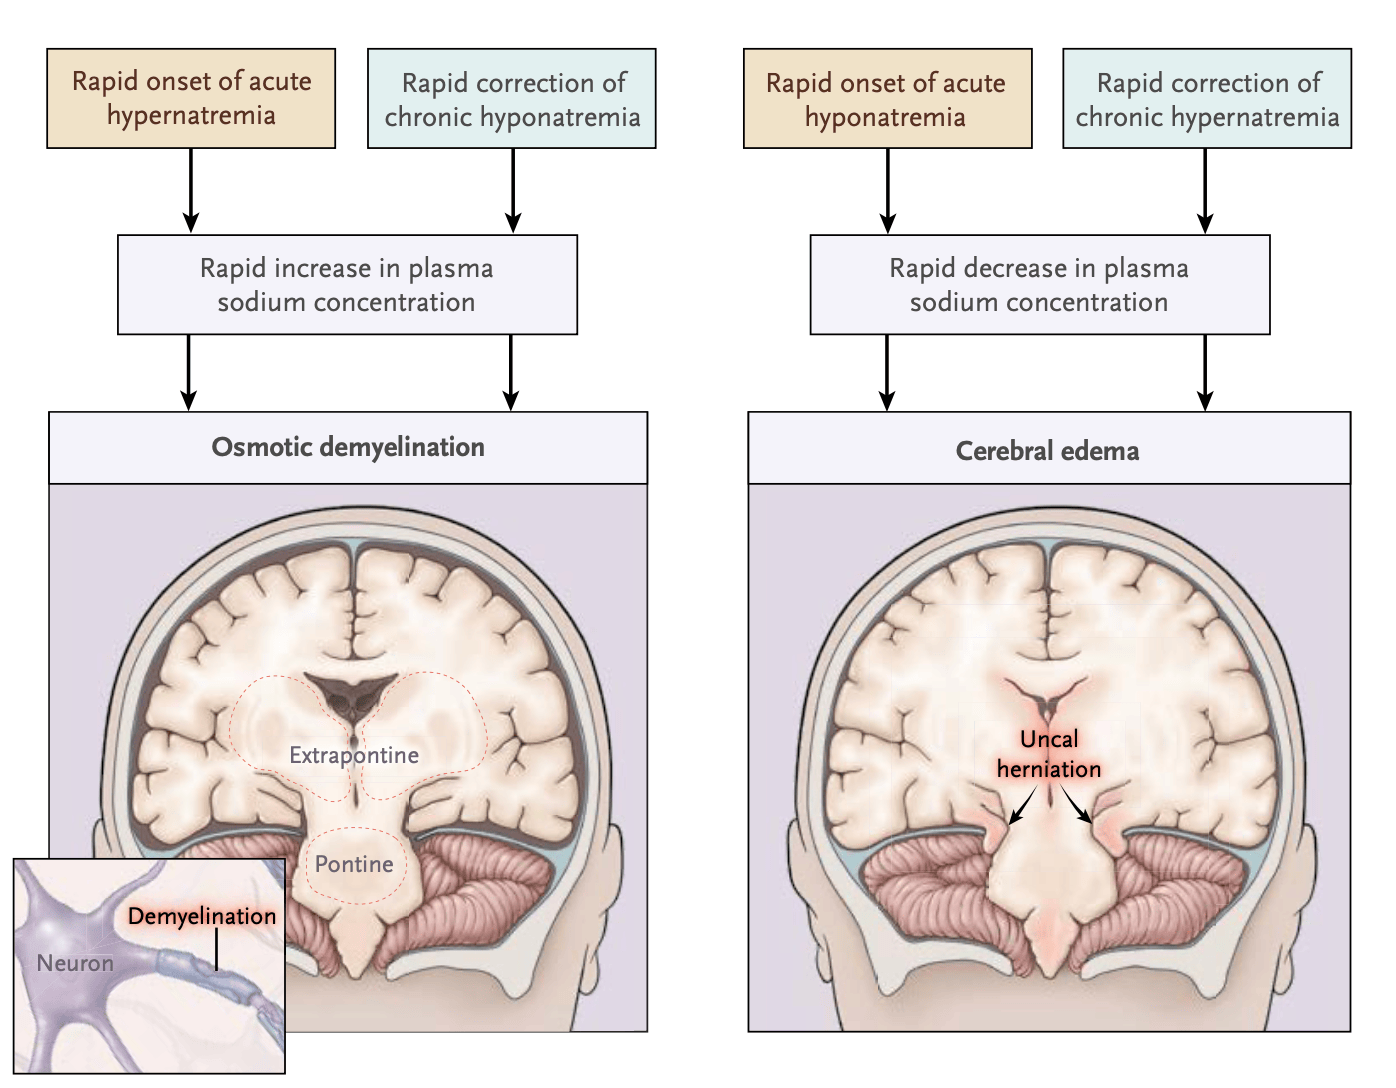
\includegraphics[width=0.8\textwidth]{pictures/fig1.png}
    \caption{Both a rapid onset and a rapid correction of hyponatremia and hypernatremia can cause brain damage. A rapid increase in the level of plasma sodium, either from acute hypernatremia or from rapid correction of chronic hyponatremia, can cause osmotic demyelination. Cerebral edema is a complication of acute hyponatremia and of rapid correction of chronic hypernatremia. Modified from Sterns\cite{sternsDisordersPlasmaSodium2015a}.}
    \label{fig1}
\end{figure}

\section{Salt disruptions, dysnatriemias in the brain injured patient}
Disturbances of plasma sodium concentrations are generally defined as dysnatriemias, those are quite common in the brain injured patient and are associated with poor neurological outcomes and mortality. Brain injury can both induce and result in dysnatriemias.\\

\textbf{Hyponatriemia} is defined as a serum sodium lower than 135 mmol/L. The highest incidence of hyponatriemia is found in subarachnoid hemorrhage (up to 60\% of patients), followed by traumatic brain injury (up to 50\% of patients). The most serious complication is defintely fatal cerebral edema and herniation.
\newline Through aquaporins water moves from the ECF to the intracellular compartment resulting in astrocytic swelling. Water is routed selectively inside glial cells to initially spare the neurons. When placed in a hyposmotic fluid, astrocytes active a mechanism known as \textit {regulatory volume decrease}. The most immediate response consists in the shifting of liquid from the interstitial space to the cerebrospinal fluid. In order to counterbalance the increase in water volume, brain cells rapidly adapt by extruding osmotically active electrolytes, this is a temporary measure as it wanes within a few hours (3 to 12 hours\cite{seayDiagnosisManagementDisorders2020a}\cite{babaApproachManagementSodium2022a}). If hyponatriemia is sustained, a second slower adaptive response begin, based on the efflux of organic solutes. At 48h from hyponatriemia onset, the efflux of inorganic solutes still results in a potentially critical 40\% increase of brain water volume\cite{babaApproachManagementSodium2022a}. The timespan required for the brain to expel more than 90\% of organic osmoles is the physiological basis for discriminating between acute (<48h) and chronic (>48h) hyponatriemia\cite{rafatHyponatremiaIntensiveCare2015a}. 
\newline Altough many conditions can lead to hyponatriemia, in the brain injured those are commonly related to the syndrome of inappropriate release of antidiuretic hormone (SIADH) and cerebral salt wasting syndrome (CSW).
\newline In SIADH, serum antidiuretic hormon levels are erroneously high, resulting in inappropiately elevated urine osmolality secondary to urinary loss of sodium, despite hyponatriemia.
\newline Cerebral sal wasting is primarily a natriuresis problem, thus euvolemia and hypervolemic state are often present in SIADH, wehereas hypovolemia is common in untreated CSW.

At the opposite end of the spectrum, \textbf{hypernatriemia} is defined as serum sodium higher than 145 mmol/L. Glial cells and neurons begin to lose water as a result of the osmotic gradient, while the brain tries to mantain a stable intracellular volume. To protect against  shrinkage, brain moves water from the cerebrospinal fluid into the interstitium, followed by early uptake of ions and late accumulation of organic osmoles. 
\newline In the brain injured patient is common to err on the hypernatriemic state, usually as result of osmotherapy for the management of cerebral edema, though can also be unintended as result of diabetes insipidus or other iatrogenic drugs.
\newline Mannitol induces hypernatriemia by increasing free water loss, while hyperonic saline directly increases plasma sodium.
\newline Central diabetes insipidus (CDI) occurs in case of vasopressin deficit or as a component of the pituitary stalk injury. Hypernatriemia may also manifest as a complication of anterior communicating aneurysm rupture or injury to anterio hypothalamus\cite{mahannaManagementSodiumAbnormalities2015a}.\\

\section[The water wars, understanding SIADH, CSW and DI]{The water wars, understanding SIADH, Cerebral Salt Wasting and Diabetes Insipidus}
In the intricate balance of fluid and electrolyte regulation, three conditions already briefly described stand out for the complex interplay in patients with brain injuries: Syndrome of Inappropriate Antidiuretic Hormone Secretion (SIADH), Cerebral Salt Wasting (CSW), and Diabetes Insipidus (DI), deserving further exploration. 
Together, these conditions represent a “water war” within the body, where misregulation of fluids and electrolytes can quickly escalate to worrisome situations.\\

The \textbf {Syndrome of Inappropriate Antidiuretic Hormone Secretion} (SIADH) - recently renamed as SIAD (syndrome of inappropriate antidiuresis) - is characterized by excessive release of antidiuretic hormone (ADH), leading to water retention and dilutional hyponatremia. This disorder is frequently encountered in neurocritical care patients, particularly following traumatic brain injury (TBI), subarachnoid hemorrhage, and neurosurgical procedures. In SIADH, the kidneys retain free water, resulting in euvolemic hyponatremia with high urine osmolality and sodium concentration. 

The diagnostic criteria include several key markers. Hyponatremia is a hallmark feature, with serum osmolality below 270-275 mOsm, indicating hypotonic plasma. Despite this, urine osmolality is typically elevated, often exceeding 300 mOsm, though values between 100-300 mOsm may place the diagnosis into question. Another important diagnostic feature is high urinary sodium concentration, which suggests that sodium is being excreted despite low plasma sodium levels. Clinically, patients with SIADH appear euvolemic, showing no signs of fluid overload or dehydration. Additionally, the hyponatremia should not be attributable to renal failure, as renal function typically remains intact unless the glomerular filtration rate (GFR) falls below 20-25 ml/min. Common treatments for SIADH involve addressing any reversible causes and promoting adequate protein and salt intake. Fluid restriction to <500-1000 ml/day can be effective in about half of patients, although often difficult.\footnote {Fluid restriction is less likely to succeed if urine osmolality is greater than 500 mOsm or urine sodium exceeds 130 mM.\cite{warrenSyndromeInappropriateAntidiuresis2023}}

For more resistant cases, oral urea is a preferred treatment, and SGLT2 inhibitors have also shown efficacy in clinical trials. Additionally, ADH inhibitors (vaptans) are also used, salt tablets may be an alternative when other treatments are contraindicated.\\

Often confused with SIADH due to overlapping clinical features, \textbf {Cerebral Salt Wasting} (CSW) is distinguished by hypovolemia caused by excessive renal sodium loss. CSW typically occurs in response to brain injury and is associated with high urinary sodium excretion and polyuria. The pathophysiology involves disruption of sympathetic pathways or increased secretion of natriuretic peptides (BNP, ANP), leading to renal salt wasting. The existence of CSW remains controversial, as it can be difficult to distinguish from SIADH due to their similar laboratory profiles. Despite conflicting reports on the prevalence of CSW, evidence suggests it may be linked to aldosterone deficiency in certain patients. Treatment generally includes hypertonic therapy for hyponatremia and isotonic fluids with fludrocortisone to correct hypovolemia, aiming to restore fluid balance. Notably, both CSW and SIADH can be managed with hypertonic saline, although their underlying mechanisms differ\cite{sternsCerebralSaltWasting2008}.\\

In contrast to SIADH and CSW, \textbf {diabetes insipidus} (DI) results from the inability to produce or respond to ADH, leading to excessive water loss and hypernatremia. DI is common in patients with severe brain injury, particularly those involving the hypothalamus or pituitary gland. This condition is marked by polyuria, low urine osmolality, and elevated serum sodium. DI is managed by replacing vasopressin activity with desmopressin (a synthetic ADH analogue) but this  carries the risk of free water retention, which can lead to rebound hyponatremia if not  monitored. A common and effective method to treat hypernatremia is the DDAVP clamp, where a high dose of desmopressin (e.g., 2 mcg IV every 8 hours) is used. However, once hypernatremia is controlled, the dose should be reduced to allow some free water excretion, thus avoiding hyponatremia\cite{macmillanDesmopressinPreventRapid2015}.\\

While SIADH, CSW, and DI all affect sodium and water balance, the primary difference lies in their impact on volume status. SIADH presents with euvolemia, CSW with hypovolemia, and DI with hypovolemia and hypernatremia. Early and accurate diagnosis is crucial in tailoring treatments to the specific disorder, as each requires a vastly different approach—fluid restriction for SIADH, fluid and salt repletion for CSW, and hormone replacement for DI. Failure to distinguish between these conditions can result in improper treatment, exacerbating brain injury and worsening outcomes.

%USARE ARTICOLO Approach to the Management of Sodium Disorders in the Neuro Critical Care Unit%plasma sodium, salt of life
\clearemptydoublepage
%% CHAPTERS
% add any further chapter file here
%underpressure
\chapter[Navigating the pressure, plasma sodium fluctuations]{Navigating the pressure, plasma sodium fluctuations}

\section {Introduction}
\clearemptydoublepage
%navigating the pressure
\chapter[Na\textsuperscript{\scriptsize+}vigating the pressure, sodium fluctuations]{Na\textsuperscript{\scriptsize+}vigating the pressure, sodium fluctuations}

\textit{The team behind this study started as a research team for a three-day datathon event in Lecco, Italy in November 2023 - the GiViTHON - endorsed by the Clinical Data Science of Istituto di Ricerche Farmacologiche Mario Negri IRCCS and Politecnico di Milano. Ten multidisciplinary teams composed of clinicians, nurses, statisticians, and biodata analysts have been challenged to respond to clinical questions and use the subset database for population selection and   key variables extractions.} 

\section {Introduction}
Traumatic brain injury (TBI) is a critical public health issue that frequently leads to long-term disabilities or death. After a TBI, the brain’s ability to regulate itself can be significantly compromised, resulting in a cascade of physiological disruptions. One of the most important of these is impaired autoregulation, which leads to instability in intracranial pressure (ICP) and compromised cerebral perfusion pressure (CPP). Consequently, cerebral blood flow can be reduced, increasing the risk of \textit{secondary brain injury} through ischemia, hypoxia, and further swelling.

The primary aim of treatment is to prevent secondary brain injury. This concept relies on distinguishing between injured brain tissue and salvageable brain tissue. While one portion of the brain may be irreversibly damaged, other areas remain viable but at risk due to inadequate blood flow or rising ICP. Failure to manage these can worsen the damage in these vulnerable regions, ultimately exacerbating the overall brain injury.\\

Dysnatriemias have already been recognized as a marker of severity of disease and related to mortality in the critically ill patient. There is however accumulating evidence that even mild abnormalities of serum sodium could be linked to disease severity and mortality, including changes within the normal range\cite{sakrFluctuationsSerumSodium2013}.

Serum sodium levels are tightly regulated in the human body, but patients with TBI are at higher risk of developing dysnatremias due to various factors such as hyperosmolar therapy, diabetes insipidus and SIADH. Both hypernatremia\cite{maggioreRelationIncidenceHypernatremia2009a}\cite{vedantamMorbidityMortalityAssociated2017a} and hyponatremia \cite{yumotoPrevalenceRiskFactors2015a} have been linked to higher mortality rates and worse outcomes in traumatic brain injury (TBI) patients as well as in aneurysmal subarachnoid hemorrhage (aSAH)\cite{labibSodiumItsImpact2024}\cite{balesEffectHyponatremiaSodium2016}, highlighting the importance of sodium regulation as a key therapeutic goal for individuals with elevated intracranial pressure. While managing serum sodium levels is important, fluctuations in sodium concentration, rather than just the absolute levels, may also  contribute to injury.\\

We therefore investigate the relationship between fluctuations in plasma sodium (deltaNa) and intracranial pressure (deltaICP) to evaluate how sodium variability influences ICP dynamics. Fluctuations are represented as time patients spent with sodium and ICP levels above or below predefined thresholds — referred to as Na Dose and ICP Dose — as well as  fluctuations within physiologic range.\\

\section {Materials and methods}
\subsection{Study population}
The cohort of critically ill patients with TBI was enrolled from a subpart of the Margherita3 electronic health record database - developed by the Italian Group for the Evaluation of Interventions in Intensive Care Medicine\cite{finazziDataCollectionResearch2018} - which contains the comprehensive clinical data of 5730\textcolor{red}{CONTROLLARE NUMERO PAZIENTI} patients of about 70 italian intensive care units (ICUs) registered between \textcolor{red}{AGGIUNGERE LE DATE}. 

The patients were searched based on the International Classification of Diseases (ICD-10) code. The inclusion criteria identified 411 \textcolor{red}{CONTROLLARE NUMERO PAZIENTI} patients who were diagnosed with TBI.

For most of the study variables, the software immediately ran an automatic check for internal consistency, generating queries then sent to physicians for resolution before incorporation of the new data into the database.\\

The inclusion criteria were as follows: (1) age $\geq$ 18 years, (2) TBI as cause of admission, (3) at least one intracranial pressure (ICP) reading, (4) at least one plasma sodium value.
The exclusion criteria were as follows: (1) expected ICU admission patients, (2) ICU admission after elective surgery, (3) ICU stay of less than 72h (20 patients). Patients who died within 72 hours of ICU admission were excluded to focus the analysis on those with potentially salvageable brain injuries.

\subsection{Data Collection}
Baseline parameters within the first day after ICU admission were collected including demographics (e.g., sex, age, weight, admission type), comorbidities (e.g., myocardial infarction, congestive heart failure, chronic pulmonary disease, and renal disease), assessment scale scores (Glasgow Coma Scale, GCS and Acute Physiologic Assessment and Chronic Health Evaluation, APACHE II Scoring System), intracranial pressure and pupil reactivity.

We gathered all serum sodium measurements from ICU admission up to 14 days, or until death, whichever occurred first. Additionally, we recorded data on various therapies, including extraventricular drainage, use of osmotherapy, barbiturate coma, hypothermia, among others. Lastly, we collected outcome data such as 14-day ICU mortality and overall ICU mortality.

The features extracted can be seen in Tables \ref{tab:categorical_features} and \ref{tab:continuous_features}.

\subsection{Generation of Variables and Definitions}

\paragraph{Serum Sodium Concentration on Admission and Na Dose}

Serum sodium concentration on admission was defined as the first available sodium measurement after admission to the Intensive Care Unit (ICU). Hyponatremia and hypernatremia were defined as conditions where at least three consecutive serum sodium values were below 135~mmol/L or above 145~mmol/L, respectively. The \textit{Na Dose} was defined as the area under the curve (AUC) where plasma sodium remains below (for hyponatremia) or above (for hypernatremia) the respective thresholds over time. This metric quantifies the extent and duration of sodium abnormalities, providing a cumulative measure of sodium imbalance.

\paragraph{Glasgow Coma Scale (GCS)}

The Glasgow Coma Scale (GCS) on admission was defined as the first available GCS score after admission to the ICU, with a specific focus on the motor component (GCSm)\cite{kouloulasPrognosticValueTimerelated2013}. Additionally, we evaluated the best GCS scores within the first 24~hours to assess the patient's neurological status over time. 

\paragraph{Intracranial Pressure (ICP) Dose}
The \textit{ICP Dose} is defined as the area under the curve (AUC) where intracranial pressure (ICP) exceeds 22 mmHg, a threshold linked to worse outcomes in traumatic brain injury. It quantifies the combined magnitude and duration of elevated ICP, offering a measure of intracranial hypertension severity.


\paragraph{Analysis of Plasma Sodium and ICP Fluctuations}

We explored the predictive value of the ratio between changes in intracranial pressure (DeltaICP) and plasma sodium (DeltaNa) - expressed as DeltaICP/DeltaNa - considering the dynamic nature of their relative changes over time. 

To achieve this, we first generated continuous curves for both Na and ICP using linear interpolation. For Na, linear interpolation was applied between the first and last available sodium concentration values obtained from ABG samples, generating interpolated values at one-minute intervals across the entire timeframe. The same interpolation process was applied to the ICP data, resulting in a continuous curve of ICP values at one-minute intervals. This step ensures a consistent temporal resolution for both variables, enabling a detailed analysis of their fluctuations.

Using a literature-based timeframe[37][30] to estimate the delay between changes in plasma sodium and corresponding changes in ICP, we applied a grid search method based on Granger causality\footnote{Granger causality is a statistical method that tests whether past values of one variable can predict future values of another. If one variable improves the prediction of another, it is said to “Granger- cause” the other.} to identify the best-fitting time difference. This optimal value ($\tau$) was then used to shift the ICP curve relative to the sodium curve. DeltaNa and DeltaICP were defined, corrispectively, as the time differences between consecutive values for both Na and ICP, based on the time-lag between the Na curve and the ICP curve (represented by the previously defined $\tau$).
%A further grid search was performed using multiple and submultiple values of the delta-time to identify the best-fitting one.

The concept of $\tau$ is crucial in this context as it represents the time delay between a change in Na (cause) and its resulting effect on ICP (effect). For instance, if we consider time points $T_0$ and $T_1$ for Na, and the same time points for ICP, it would be incorrect to directly correlate these changes without accounting for the time it takes for a change in Na to affect ICP. 


%To determine the optimal $\tau$, we initially employed Granger causality analysis, a statistical method that assesses whether past values of one time series can predict future values of another. This step served to confirm the well-established directional relationship where changes in Na levels influence subsequent changes in ICP (Na $\rightarrow$ ICP) as documented in the literature. However, while Granger causality validated the direction of influence, it \textit{did not provide a statistically significant universal value for} $\tau$ across the patient population. This finding indicated that a fixed $\tau$ could not adequately describe the relationship for all patients.

%Given this limitation, we adopted an empirical approach using a grid search to identify the optimal $\tau$ for each patient. The grid search involved testing various $\tau$ values within a plausible range based on clinical knowledge and previous studies \textcolor{blue}{Ti va se mettiamo proprio i valori?} For each $\tau$ value tested, the Na and ICP curves were aligned accordingly, and we evaluated which alignment produced a dataset that resulted in the best performance of downstream machine learning (ML) models. This data-driven method allowed us to select the most appropriate $\tau$ for each patient, taking into account individual variability in the time delay between changes in Na and their effects on ICP.

By selecting the $\tau$ that maximized the predictive accuracy of the ML models, we ensured that the time-series alignment was optimized for subsequent analysis. This iterative optimization provided a tailored approach for each patient, enhancing the reliability of the calculated DeltaICP/DeltaNa values and their use in predicting patient outcomes.

%In summary, the procedure involved generating interpolated time-series data for Na and ICP, confirming the Na $\rightarrow$ ICP relationship with Granger causality, and using a grid search approach to empirically determine the optimal $\tau$ for aligning these curves. By validating that \(\frac{\Delta \text{ICP}}{\Delta \text{Na}}\) contains relevant and essential information for predicting outcomes, we emphasize its potential value for informing ICU treatment decisions.

Once the curves were aligned using the optimal time delay ($tau$), it was necessary to select a time interval, referred to as "delta time," for calculating the differences between consecutive samples in both the sodium (Na) and intracranial pressure (ICP) curves. The delta time represents the time interval between each sample point and its preceding one, which determines the granularity of the observed changes (DeltaNa and DeltaICP). 
A further grid search was performed for the delta-time to identify the best-fitting one, starting from multiple or submultiple of the tau value.

\subsection{Therapy Intensity Level}
\textcolor{red}{DA FINIRE}
We  divided the patients into three subgroups based on their maximum TIL (Therapy Intensity Level) reached during the observation window. The TILs were simplified from the stepwise therapy and therapeutic TILs proposed in other studies. A more detailed categorisation wasn’t possible due to the absence of certain key variables in the dataset (such as decompressive craniectomy and hypertonic solution therapy). See Table \ref{tabTIL}

\begin{table}[h!]
    \centering
    \renewcommand{\arraystretch}{1.5} % Adjust the row height
    \begin{adjustbox}{width=0.8\textwidth}
    \begin{tabular}{|>{\raggedright\arraybackslash}p{4cm}|>{\raggedright\arraybackslash}p{4cm}|>{\raggedright\arraybackslash}p{10cm}|}
        \hline
        \textbf{Categorized TIL} & \textbf{TIL SCALE} & \textbf{DESCRIPTION} \\
        \hline
        \multirow{2}{*}{\textbf{TIL 1}} 
        & \textbf{No specific therapy} & No specific ICP directed therapy \\
        \cline{2-3}
        & \textbf{Basic} 
        & - Sedation for ventilator/endotracheal tube tolerance* \newline 
        - Volume/vasopressors for non-cerebral nervous system cause (e.g., sepsis, myocardial injury)** \newline 
        - Head-up positioning (ventilator bundle) \newline 
        - Normocapnia (partial pressure of carbon dioxide PaCO$_2$ ≥ 40 mmHg) \\
        \hline
        \multirow{2}{*}{\textbf{TIL 2-3}} 
        & \textbf{Mild} 
        & - Higher levels of sedation* \newline 
        - Vasopressors/volume for cerebral perfusion pressure (CPP) support** \newline 
        - Low dose osmotic therapy*** \newline 
        - Mild hypocapnia (PaCO$_2$ 35-40 mmHg) \newline 
        - Cerebrospinal fluid (CSF) drainage < 120 ml/day (<5 ml/hour) \\
        \cline{2-3}
        & \textbf{Moderate} 
        & - Higher doses of osmotic therapy*** \newline 
        - Moderate hypocapnia (PaCO$_2$ 30-35 mmHg) \newline 
        - Mild hypothermia ($T>35^\circ\text{C}$)) \newline 
        - CSF drainage ≥ 120 ml/day (>5 ml/hour) \\
        \hline
        \textbf{Extreme TIL (eTIL)} 
        & \textbf{Extreme} 
        & - Profound hypocapnia (PaCO$_2$ <30 mmHg) \newline 
        - Extreme hypothermia ($T<35^\circ\text{C}$) \newline 
        - Extreme suppression for ICP control \newline 
        - \st{Secondary decompression (surgery after 24h)} \\
        \hline
    \end{tabular}
    \end{adjustbox}
    \caption{Therapy Intensity Levels (TIL) scale. \footnotesize{Adapted from Robba et. al\cite{robbaTreatmentsIntracranialHypertension2023a}}}
    \small{\flushleft{No information about secondary decompression is available in the database\\$^*$ not possible to differentiate the target of sedation \\$^{**}$ not possible to differentiate the target of vasopressor therapy\\$^{***}$ about osmotic therapy, no information about the dose was available}
    \label{tabTIL}
\end{table}

\subsection{Outcome definition}
The main purpose of this study was to explore the relationship between plasma sodium and intracranial pressure on the outcome of a patient. 

For the machine learning development, a binary outcome has been defined: \textit{alive at 14 days} or \textit{not alive at 14 days}.

Then, in the subgroup analysis, we tried refining the outcome in three subclasses (alive with GCS>8, alive with GCS<8 and death) to grossly explore the neurologic status at 14 days. Both Glasgow Outcome Coma Scale and survival status at discharge were not available in the dataset.

%\subsection{Dataset internal validation}
%To prove the recognized causal relationship between sodium and ICP, we tested it using the Granger Causality method


\subsection{Machine learning models development}
In this section the predictive capabilities of different machine learning algorithms (ML models) have being tested on our dataset.

In particularly, the outcome at 14 days (target variable) was considered.
This outcome is binary, expressed as \textit{alive at 14 days} or \textit{not alive at 14 days}.

For each specific binary classification task, to gain as much as possible predictive capabilities, we tested different pipelines using as evaluation metrics the accuracy and the AUC-ROC.
Each pipeline is composed by a scaler\footnote{preprocessing tool in machine learning used to standardize or normalize feature values to ensure that each feature contributes equally to the model by bringing all values into a comparable range}, a feature selection method\footnote {technique used to identify and select the most relevant features (variables) from a dataset with the the highest predictive power to improve performance by reducing noise and avoiding overfitting.} and a machine learning model.
\begin{itemize}
	\item The base model (\textit{Model 1}) has been developed and trained starting from patient demographics and clinical features available comprehensive of summary statics of sodium trends. 
\end{itemize}

Above this base model further features where added, in order:

\begin{itemize}
	\item \textit {Model 2} accounts for the cumulative effect of ICP Dose and Na Dose. As middle step,  both ICP Dose and Na Dose were evaluated individually and then added together.
	\item The third model (\textit{Model 3}) explores the effects of the DeltaICP/DeltaNa informations over the base model. The DeltaICP/DeltaNa features where extracted as outlined in paragraph 3.2.3. 
\end{itemize}

\section {Results}
\subsection{Patient Demographics and Clinical Features}
In this section we present the descriptive characteristics of our population, divided into  categorical variables and numerical (continuous) variables.

\textcolor{red}{TO DO: SISTEMARE DESCRIZIONE TABELLE}

\begin{table}[h!]
	\centering
	\small % Reduce font size
	\begin{tabular}{lll}
		\hline
		\textbf{Feature} & \textbf{Category} & \textbf{Count\_n (\%)} \\
		\hline
		SEX & M & 321 (78.10\%) \\
		%SEX & F & 90 (21.90\%) \\
		TYPE & Chirurgico d’urgenza & 229 (55.72\%) \\
		TYPE & Medico & 182 (44.28\%) \\
		OUTCOME & alive at 14 days & 357 (86.86\%) \\
		%dividere tra alive GCS>8, alive GCS<=8 e death 
		% GCS & > 8 & xx (xx\%) \\ 
		% GCS & =< 8 & 54 (13.14\%) \\
		PUPIL & anisocorìa & 217 (52.80\%) \\
		%PUPIL & False & 194 (47.20\%) \\
		%ICPm & True & 372 (90.51\%) \\
		%ICPm & False & 39 (9.49\%) \\
		%ICPm non ho proprio capito cosa sia...
		Hypernatremia & True & 259 (63.02\%) \\ 
		%Hypernatremia & False & 152 (36.98\%) \\
		Hyponatremia & True & 154 (37.47\%) \\
		%Hyponatremia & False & 257 (62.53\%) \\
		\hline
	\end{tabular}
	\caption{Categorical Feature Statistics}
	\label{tab:categorical_features}
\end{table}

\begin{table}[h!]
	\centering
	\tiny % Reduce font size
	\begin{tabular}{lcc}
		\hline
		\textbf{Feature} & \textbf{Mean (unit)} & \textbf{Range (unit)}\textcolor{blue}{[mean-std, mean+std]} \\ \hline
		Altezza & 173.24 (cm) & [160.63 - 185.86] (cm) \\
		Peso & 81.53 (kg) & [66.77 - 96.28] (kg) \\
		BMI & 25.46 (kg/m$^2$) & [21.31 - 29.61] (kg/m$^2$) \\
		Best GCS during first 24h hours & 6.29 & [3 - 9.84] \\
		%Worst GCS \textcolor{red}{at admission} & 2.41 & 3.14 & [-0.74 - 5.55] \\
		Best GCS Motor response during first 24h hours & 3.05 & [1.13 - 4.97] \\
		%Worst\_GCS\_Motor\_Response & 1.43 & 1.44 & [-0.01 - 2.88] \\
		
		AGE  & 54.83 (years) & [36.75 - 72.90] (years) \\
		APACHE II Score & 27.46& [22.64 - 32.29] \\
		First Sodium Value & 139.59 (mmol/L)  & [135.11 - 144.07] (mmol/L) \\
		Time to Hypernatremia & 48.97 (h)  & [5.95 - 91.99] (h) \\
		Time to Hyponatremia & 55.32 (h)  & [0 - 111.96] (h) \\
		%Na min first 7 days & 135.12 (mmol/L) & 8.76 (mmol/L) & [126.36 - 143.88] (mmol/L) \\
		%Na max first 7 days & 148.33 (mmol/L) & 6.76 (mmol/L) & [141.57 - 155.09] (mmol/L) \\
		%li ricalcolerei come n di pazienti <135 e >145 includendoli in time to hypenatriemia e tyime to hyponatriemia OPPURE LI LASCIAMO aggiungendo comunque i dati di sopra... - vanno SU 14 GIORNI
		Na min first 14 days  & 135.11 (mmol/L)  & [126.35 - 143.87] (mmol/L) \\
		Na max first 14 days  & 148.33 (mmol/L)  & [141.57 - 155.87] (mmol/L) \\
		Na SD first 14 days & 3.53 (mmol/L)  & [1.08 - 5.97] (mmol/L) \\
		%la Na SD altri studi la chiamano Na variability, forse lascerei cosi che genera confusione, va messu anche lui su 14 giorni
		\hline
	\end{tabular}
	\caption{Continuous Feature Statistics. \footnotesize{APACHE: Acute Physiology and Chronic Health Evaluation, BMI: Body Mass Index, GCS: Glasgow Coma Scale, Na max: maximum serum sodium over 14 days, Na min: minimum serum sodium over 14 days, Na SD: standard deviation of plasma sodium over 14 days}}
	\label{tab:continuous_features}
\end{table}

\textcolor{red}{SPOSTARE OUTCOME E TIL PRIMA DEI MODELLI? CONCETTUALMENTE PIU CORRETTO?}


%\subsection{Relationship between serum sodium fluctuations and intracranial pressure}
%\textcolor{red}{VALUTARE INSIEME SE E COME HA SENSO INSERIRE QUESTO PARAGRAFO, IN RIFERIMENTO A QUEL 60\% CIRCA}
\subsection{Relationship of patient descriptives on outcome}
Our reference \textit{Model 1} achieved an AUC of 0,72 considering the patient baseline characteristics (eg. age, sex, weight, body mass index) and comorbidities (comprehensive of APACHE II score) as well as sodium-related summary statistics (min Na, max Na, Na SD, first sodium value, hypernatremia, hyponatremia, time to hypernatremia, time to hyponatremia) or neurologic status descriptive of the first 24hours (ICP monitoring, pupil status, best GCS and best motor GCS).
\begin{figure}[h]
    \centering
    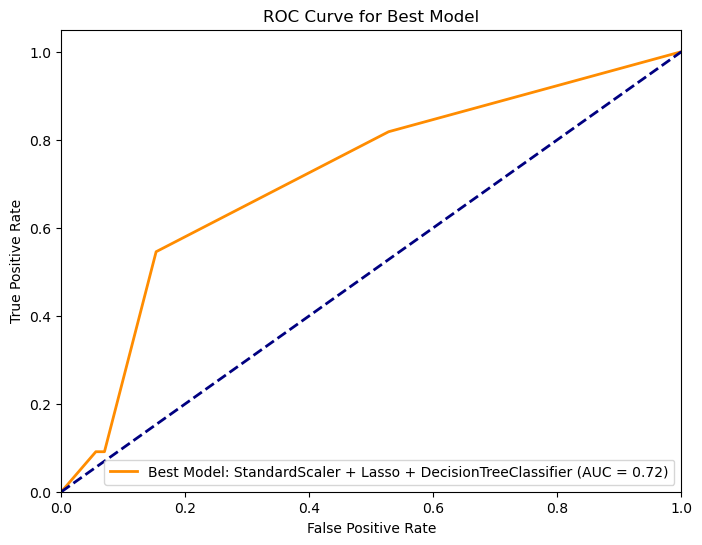
\includegraphics[width=0.6\textwidth]{pictures/fig5_basemodel.png}
    \caption{Reference model} % Add a meaningful caption
    \label{fig:model1} % Add a label for referencing
\end{figure}

\subsection{Relationship Between Na Dose and ICP Dose on outcome}
Our \textit{Model 2} achieved an AUC of 0,85 with a net 18\% improvement over base model. Additionally, over patient descriptives, this model contains informations regarding Na Dose (both above and below thresholds) and ICP Dose.

\begin{figure}[h]
    \centering
    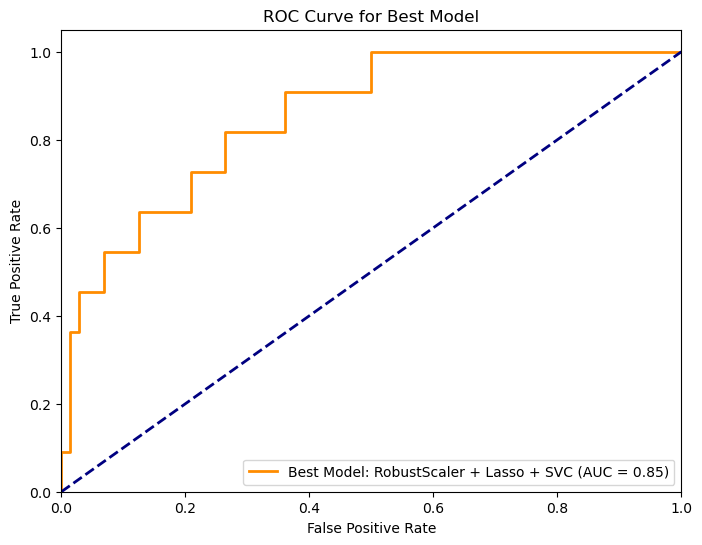
\includegraphics[width=0.6\textwidth]{pictures/fig6_model2.png}
    \caption{Model 2} % Add a meaningful caption
    \label{fig:model2} % Add a label for referencing
\end{figure}

\subsection{Relationship between sodium fluctuations and ICP fluctuations (DeltaICP/DeltaNa) on outcome}
Our last model, \textit{Model 3} was targeting the relative changes between ICP curves and sodiumc curves over time. It reached an AUC of 0,83 with a 15\% gain  over base model. 

The model 3 is the result of a grid-search testing different tau and delta times, as shown in Figure \ref{fig:model3tau}.

\begin{figure}[h]
    \centering
    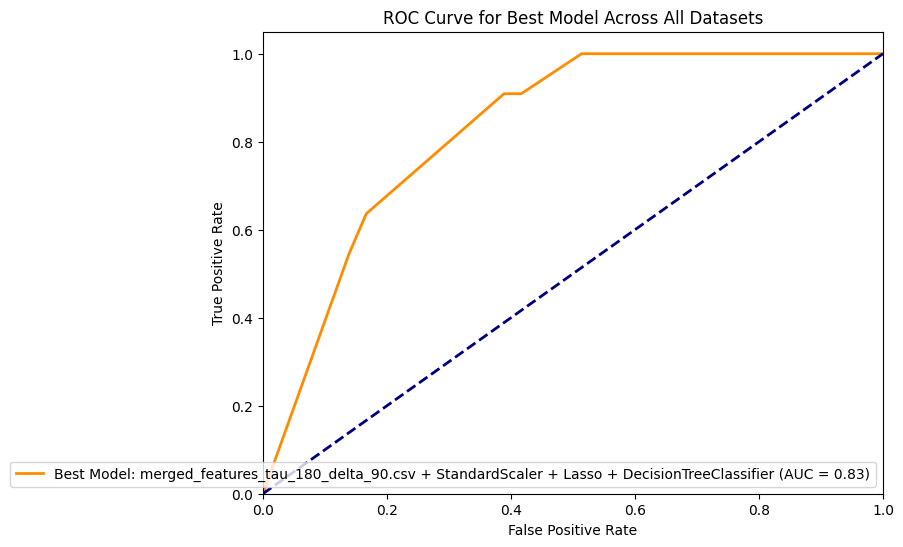
\includegraphics[width=0.8\textwidth]{pictures/fig7_model3.png}
    \caption{Model 3} % Add a meaningful caption
    \label{fig:model3} % Add a label for referencing
\end{figure}
\begin{figure}
	\centering
	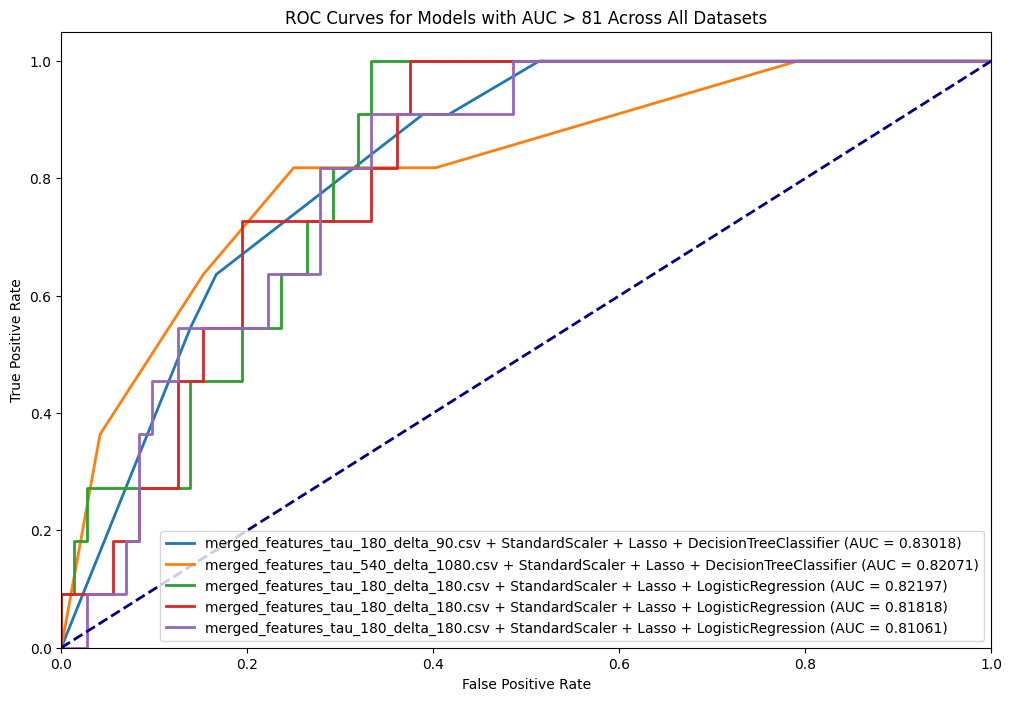
\includegraphics[width=0.8\textwidth]{pictures/fig8_model3tau.png}
	\caption{Testing different combinations with grid search, only AUC>81\% are plotted} % Add a meaningful caption
    \label{fig:model3tau} % Add a label for referencing
\end{figure}


\subsection{Subgroup analysis: outcome}

\begin{figure}[h!]
    \centering
    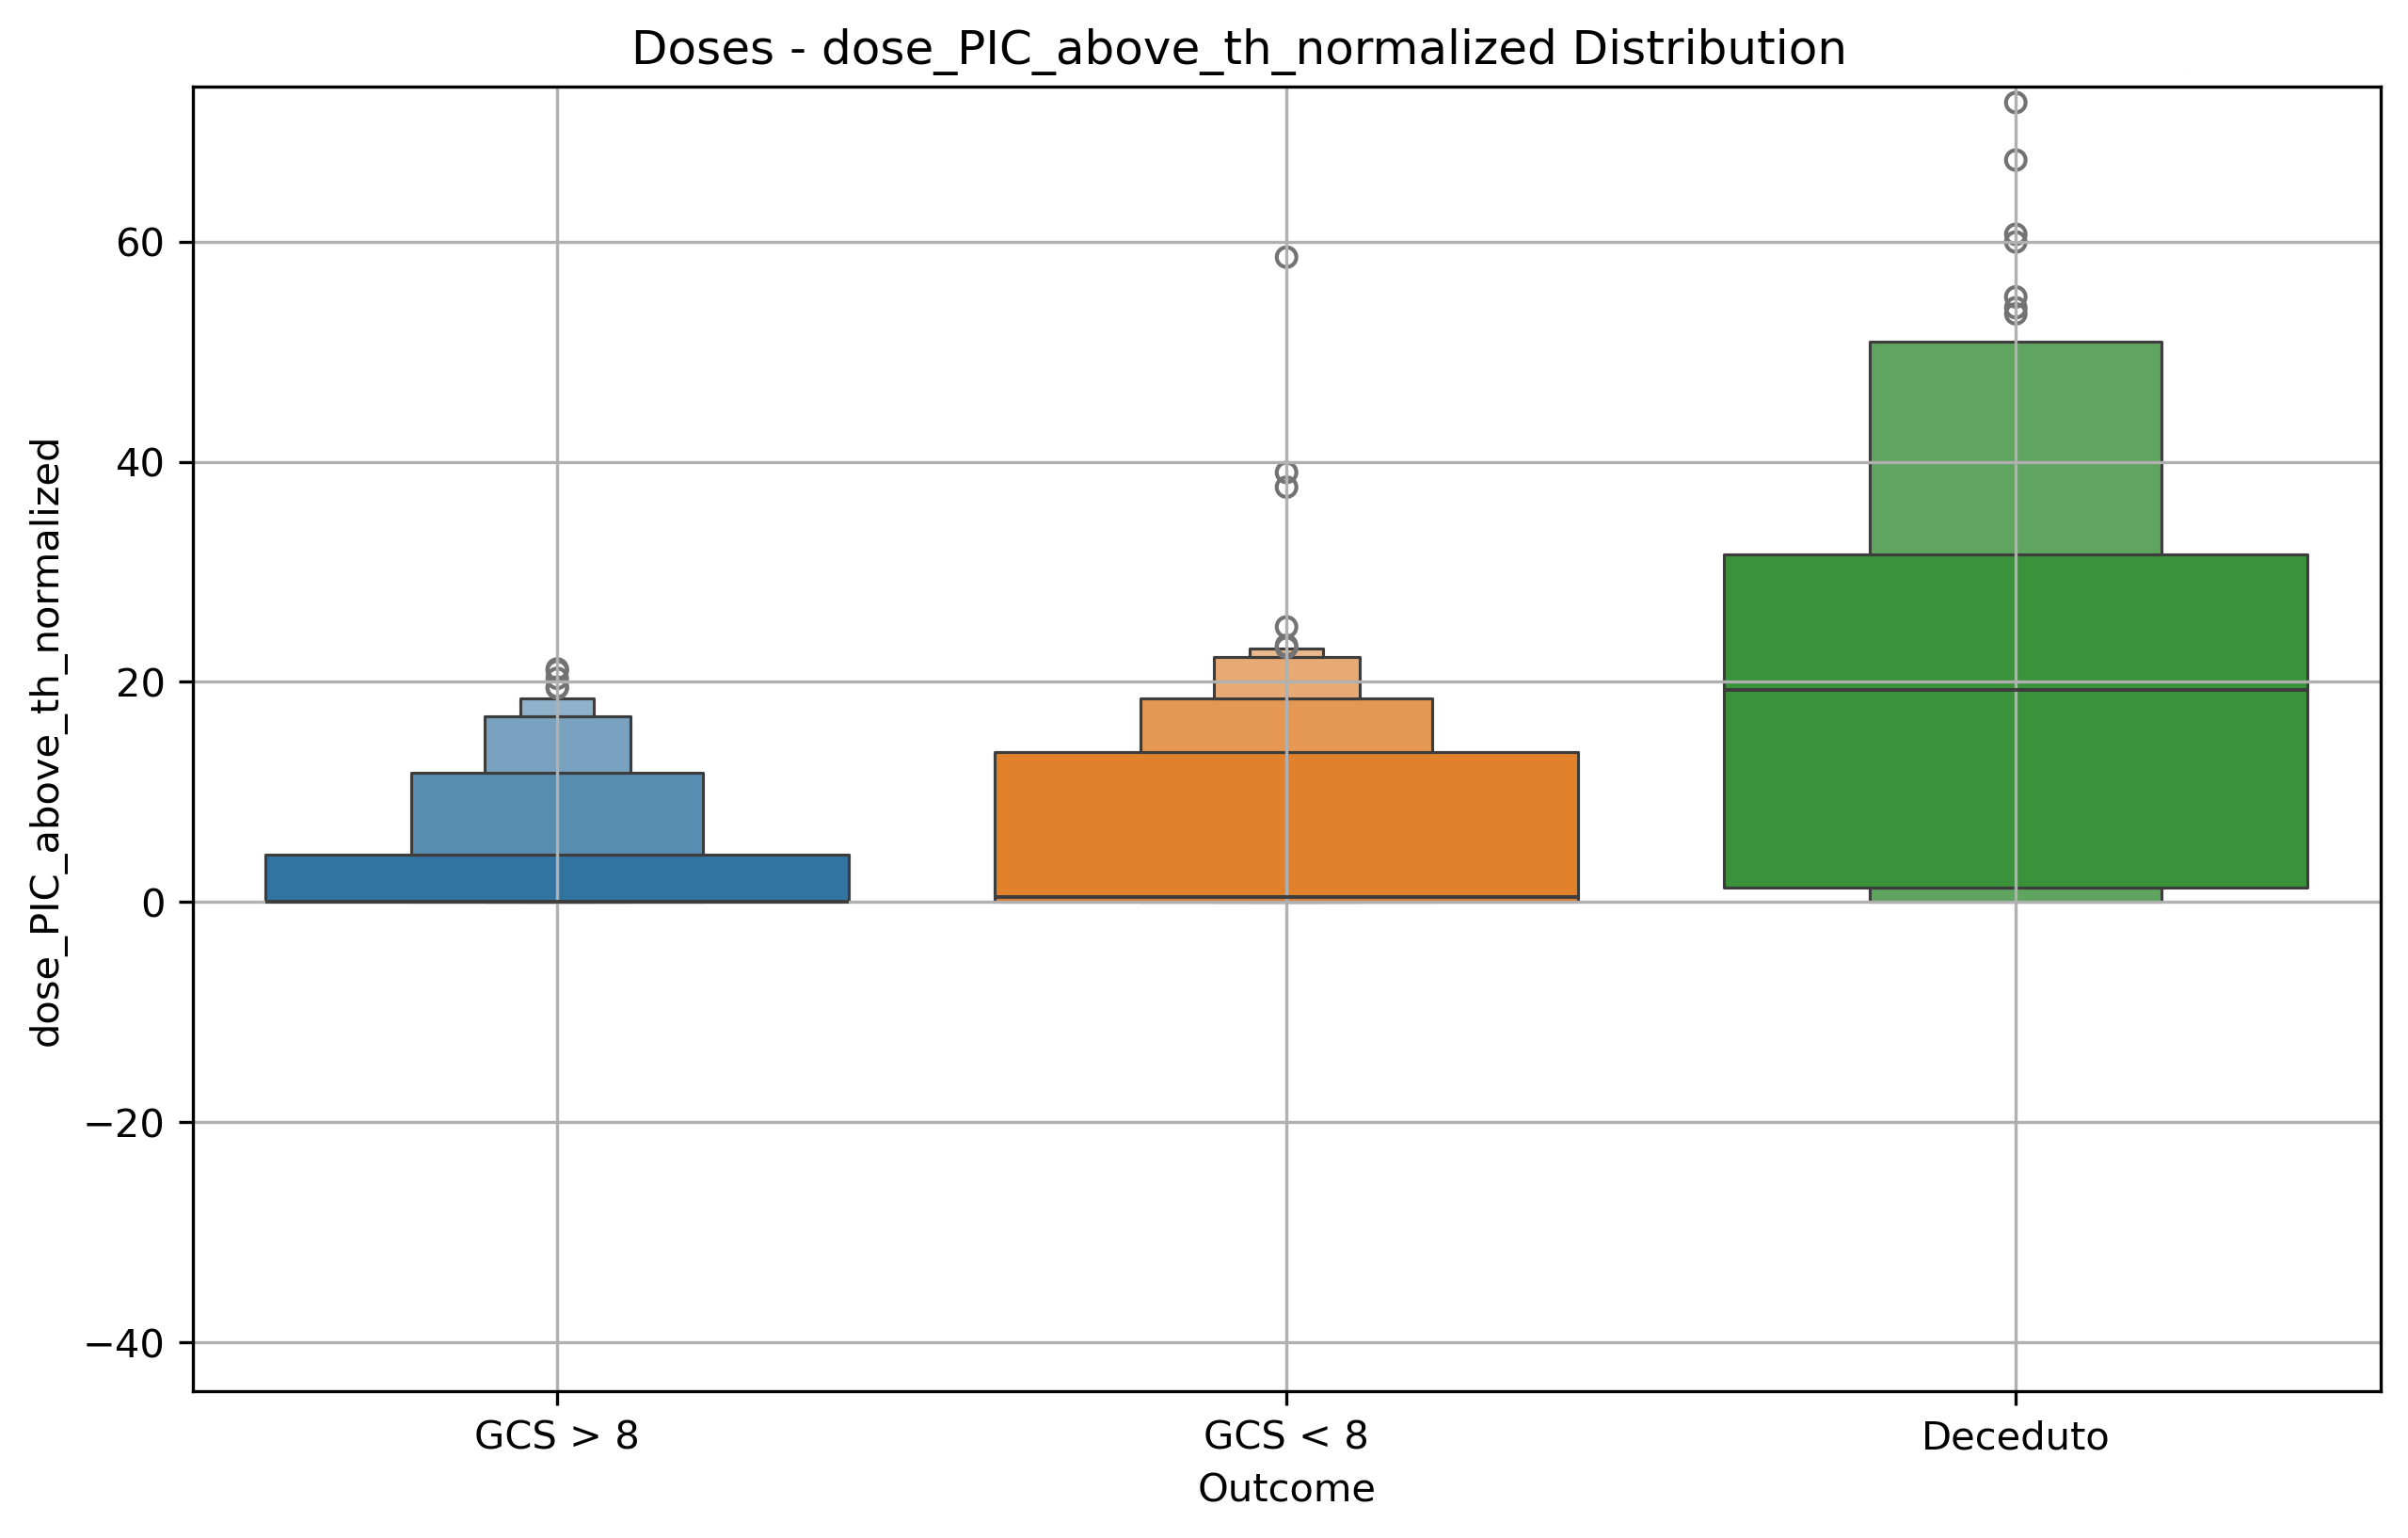
\includegraphics[width=0.8\textwidth]{pictures/fig9_ICPdose.png}
    \caption{ICP Dose and outcome} % Add a meaningful caption
    \label{fig:ICPdose_outcome} % Add a label for referencing
\end{figure}

\begin{figure}[h!]
    \centering
    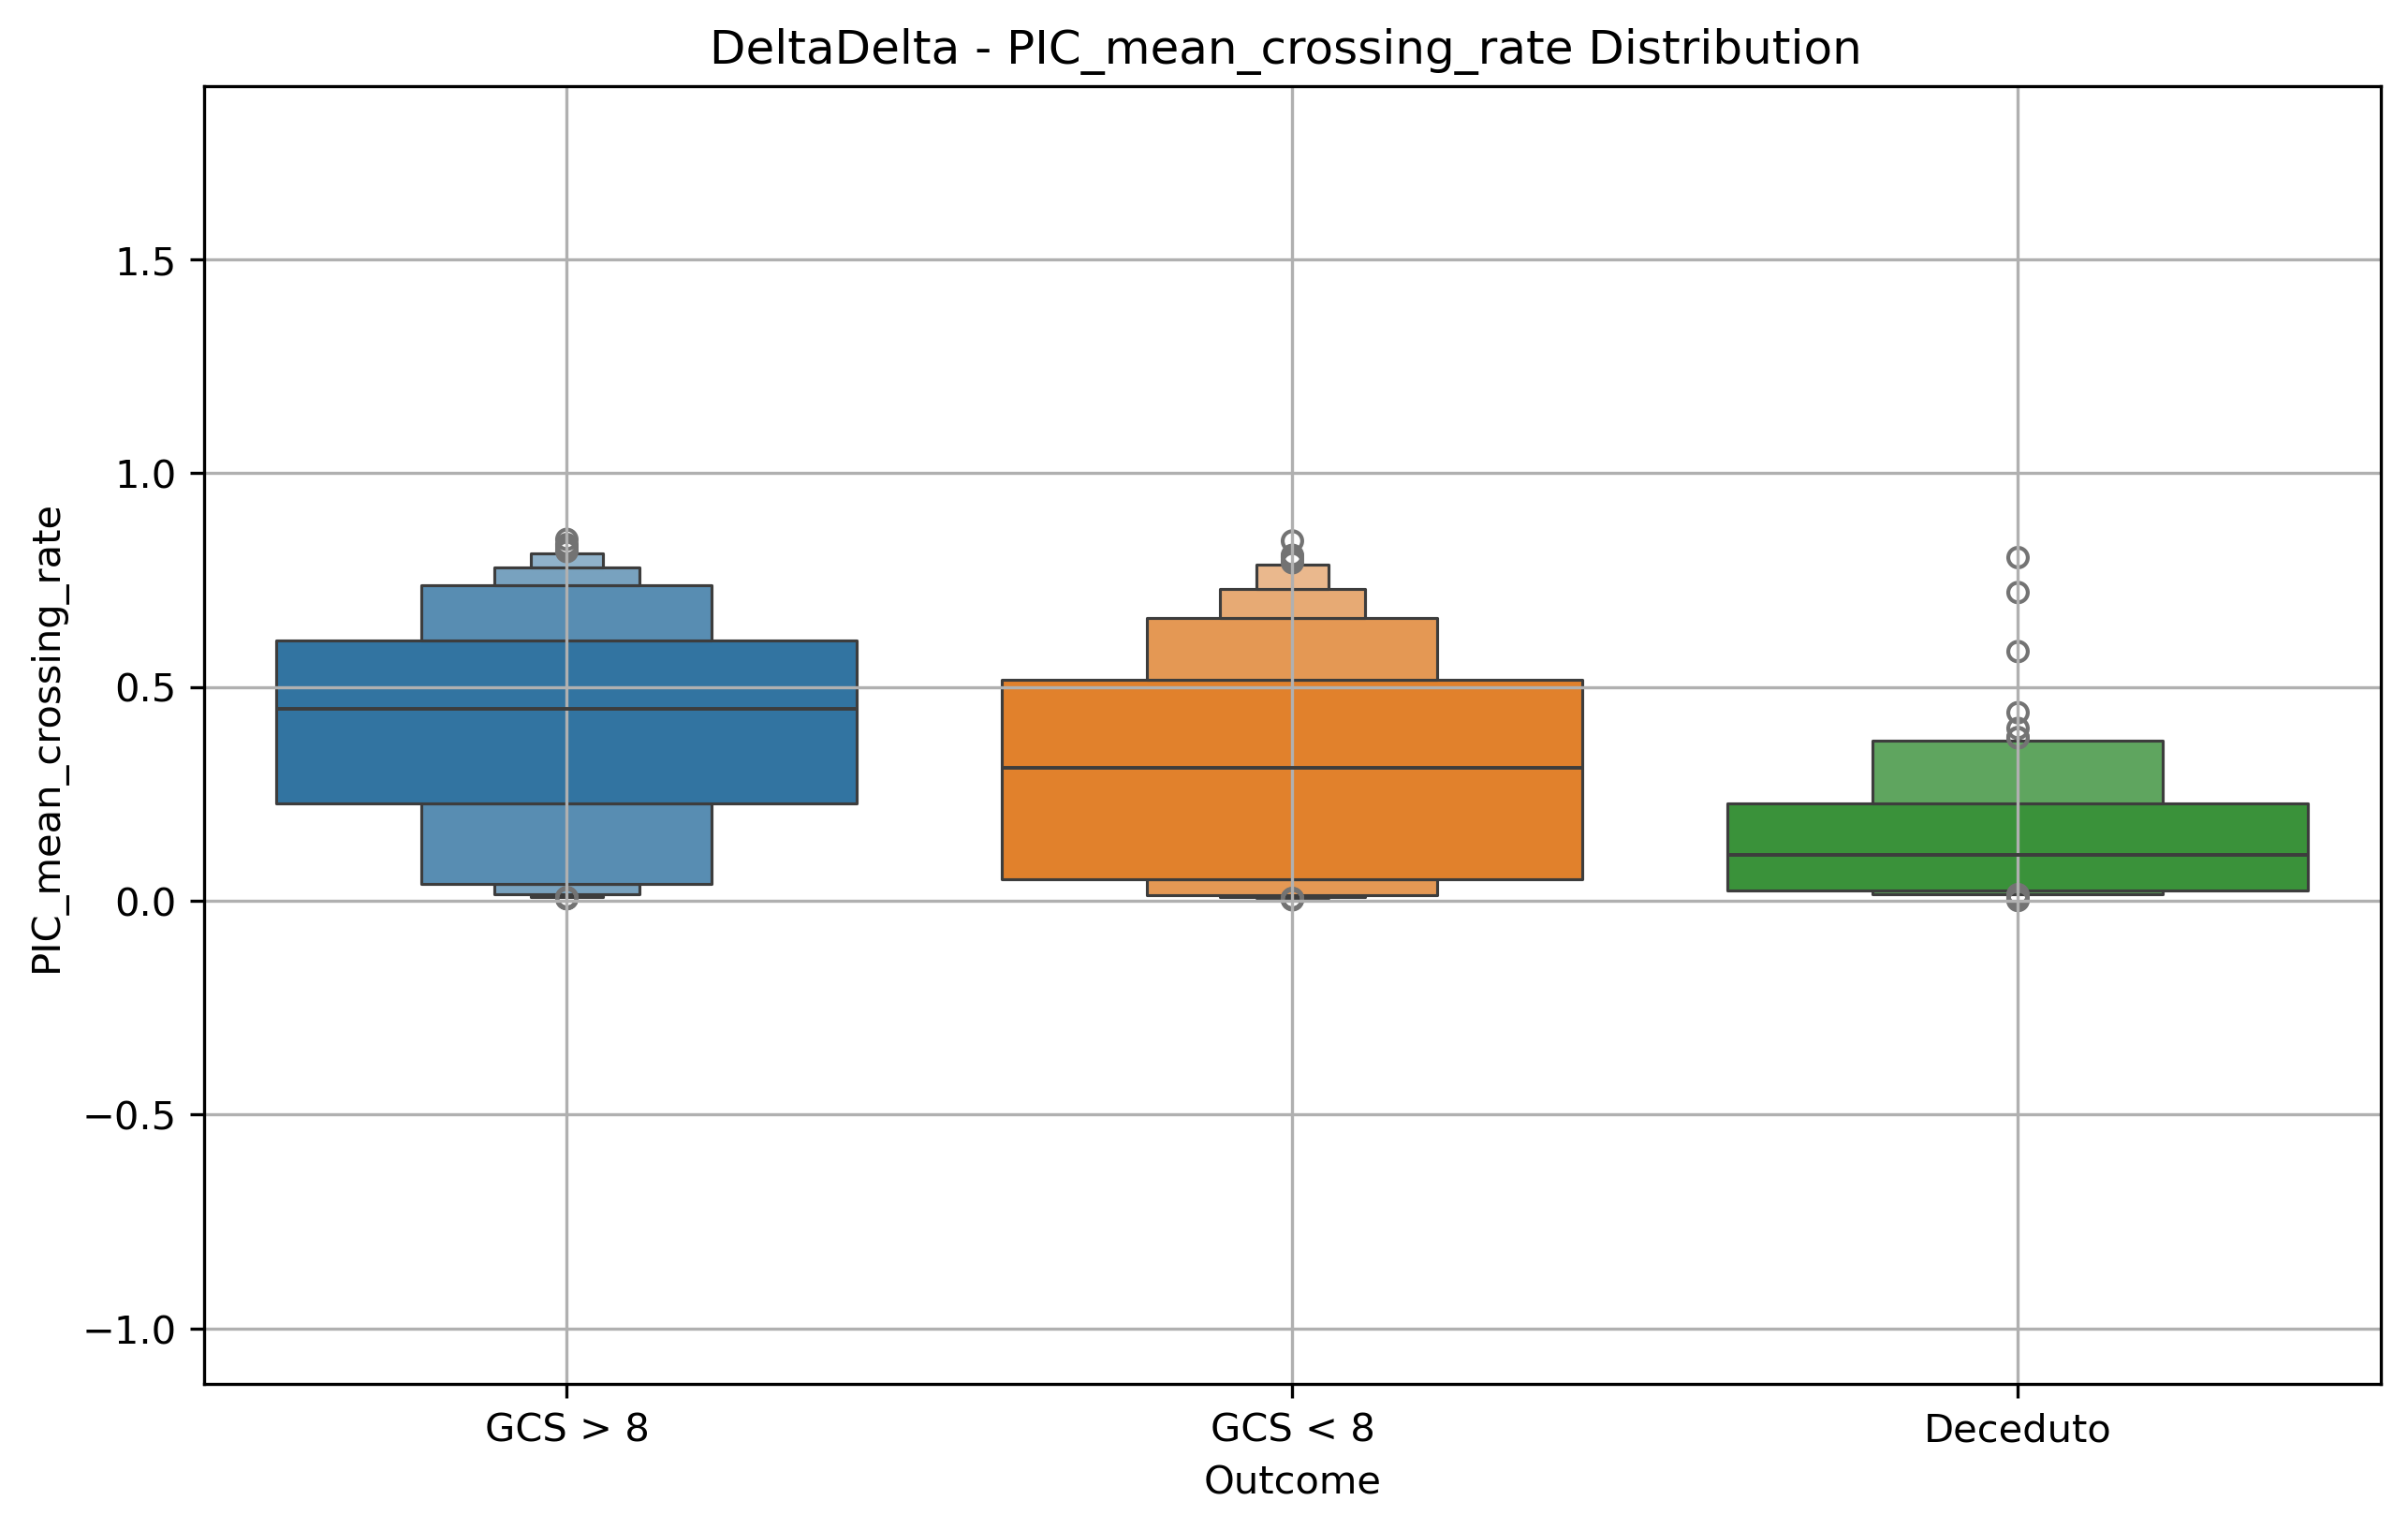
\includegraphics[width=0.8\textwidth]{pictures/fig10_ICPfluctuations.png}
    \caption{ICP fluctuations and outcome} % Add a meaningful caption
    \label{fig:ICPfluctuations_outcome} % Add a label for referencing
\end{figure}

\begin{figure}[h!]
    \centering
    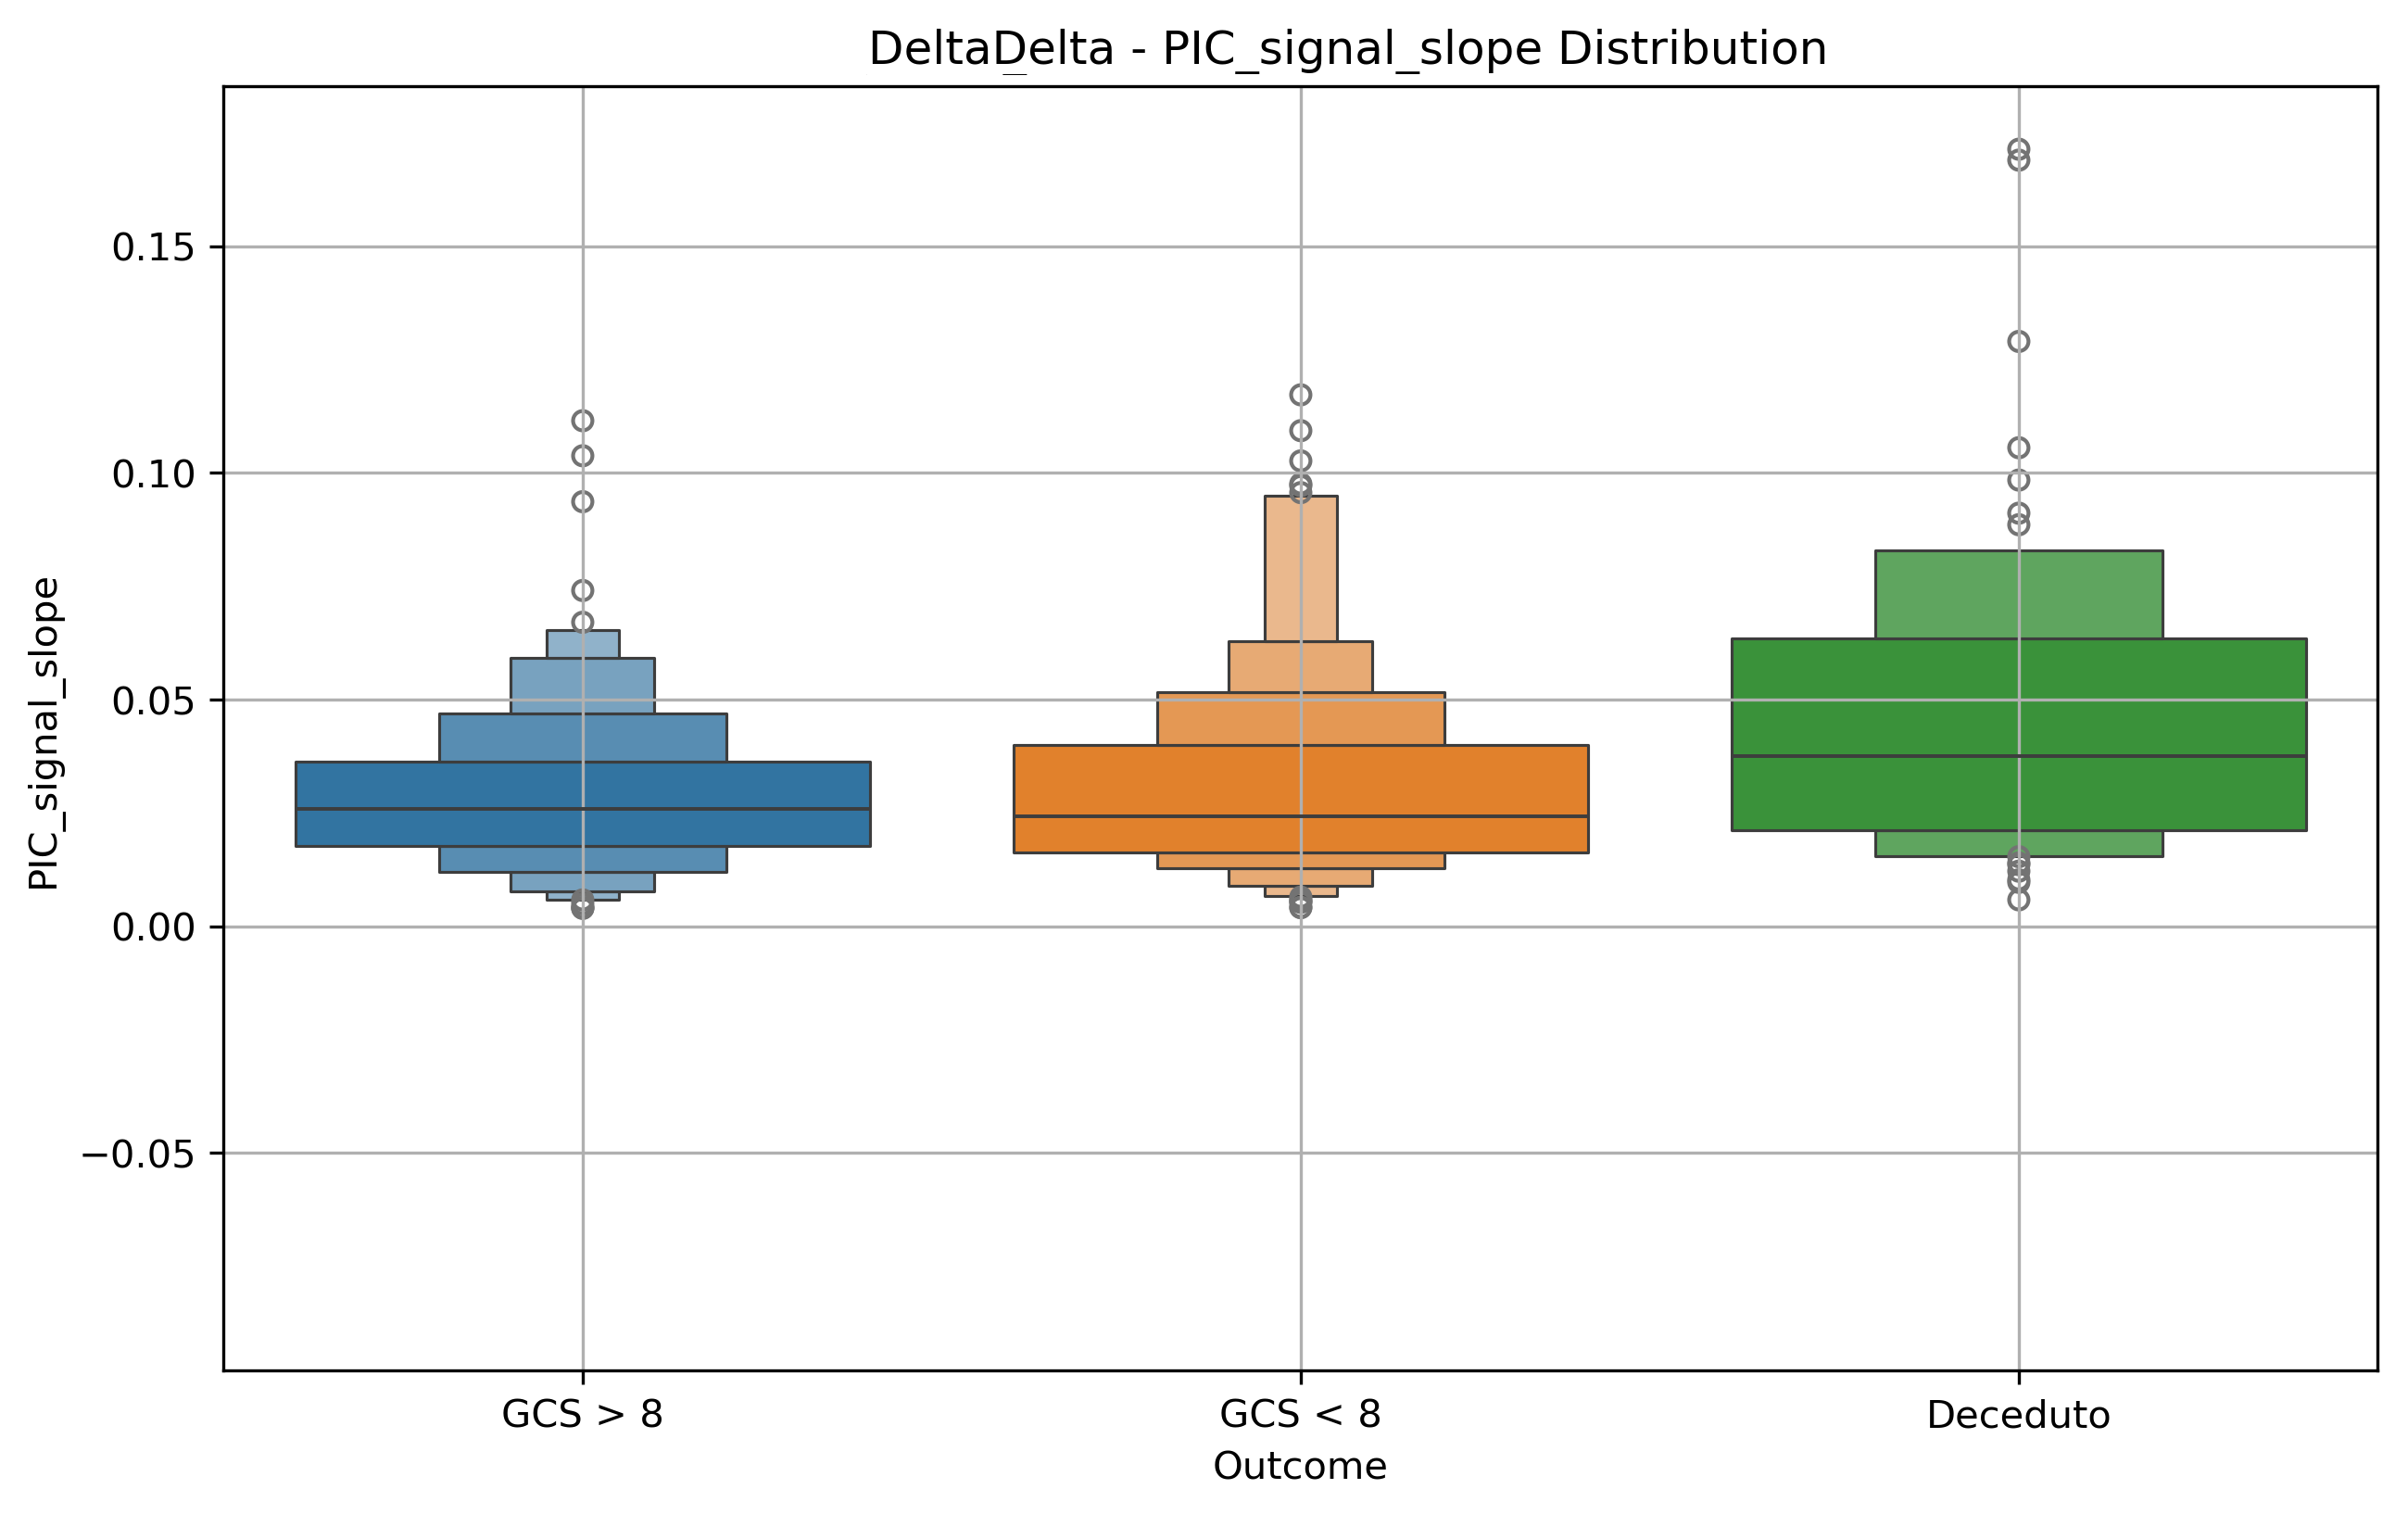
\includegraphics[width=0.8\textwidth]{pictures/fig11_ICPslope.png}
    \caption{ICP linear trend over time and outcome} % Add a meaningful caption
    \label{fig:ICPslope_outcome} % Add a label for referencing
\end{figure}

\subsection{Subgroup analysis: TIL}
\textcolor{red}{SAREBBE IL DISCORSO SUI TIL CON LE VARIE TABELLE}

\begin{figure}[h!]
    \centering
    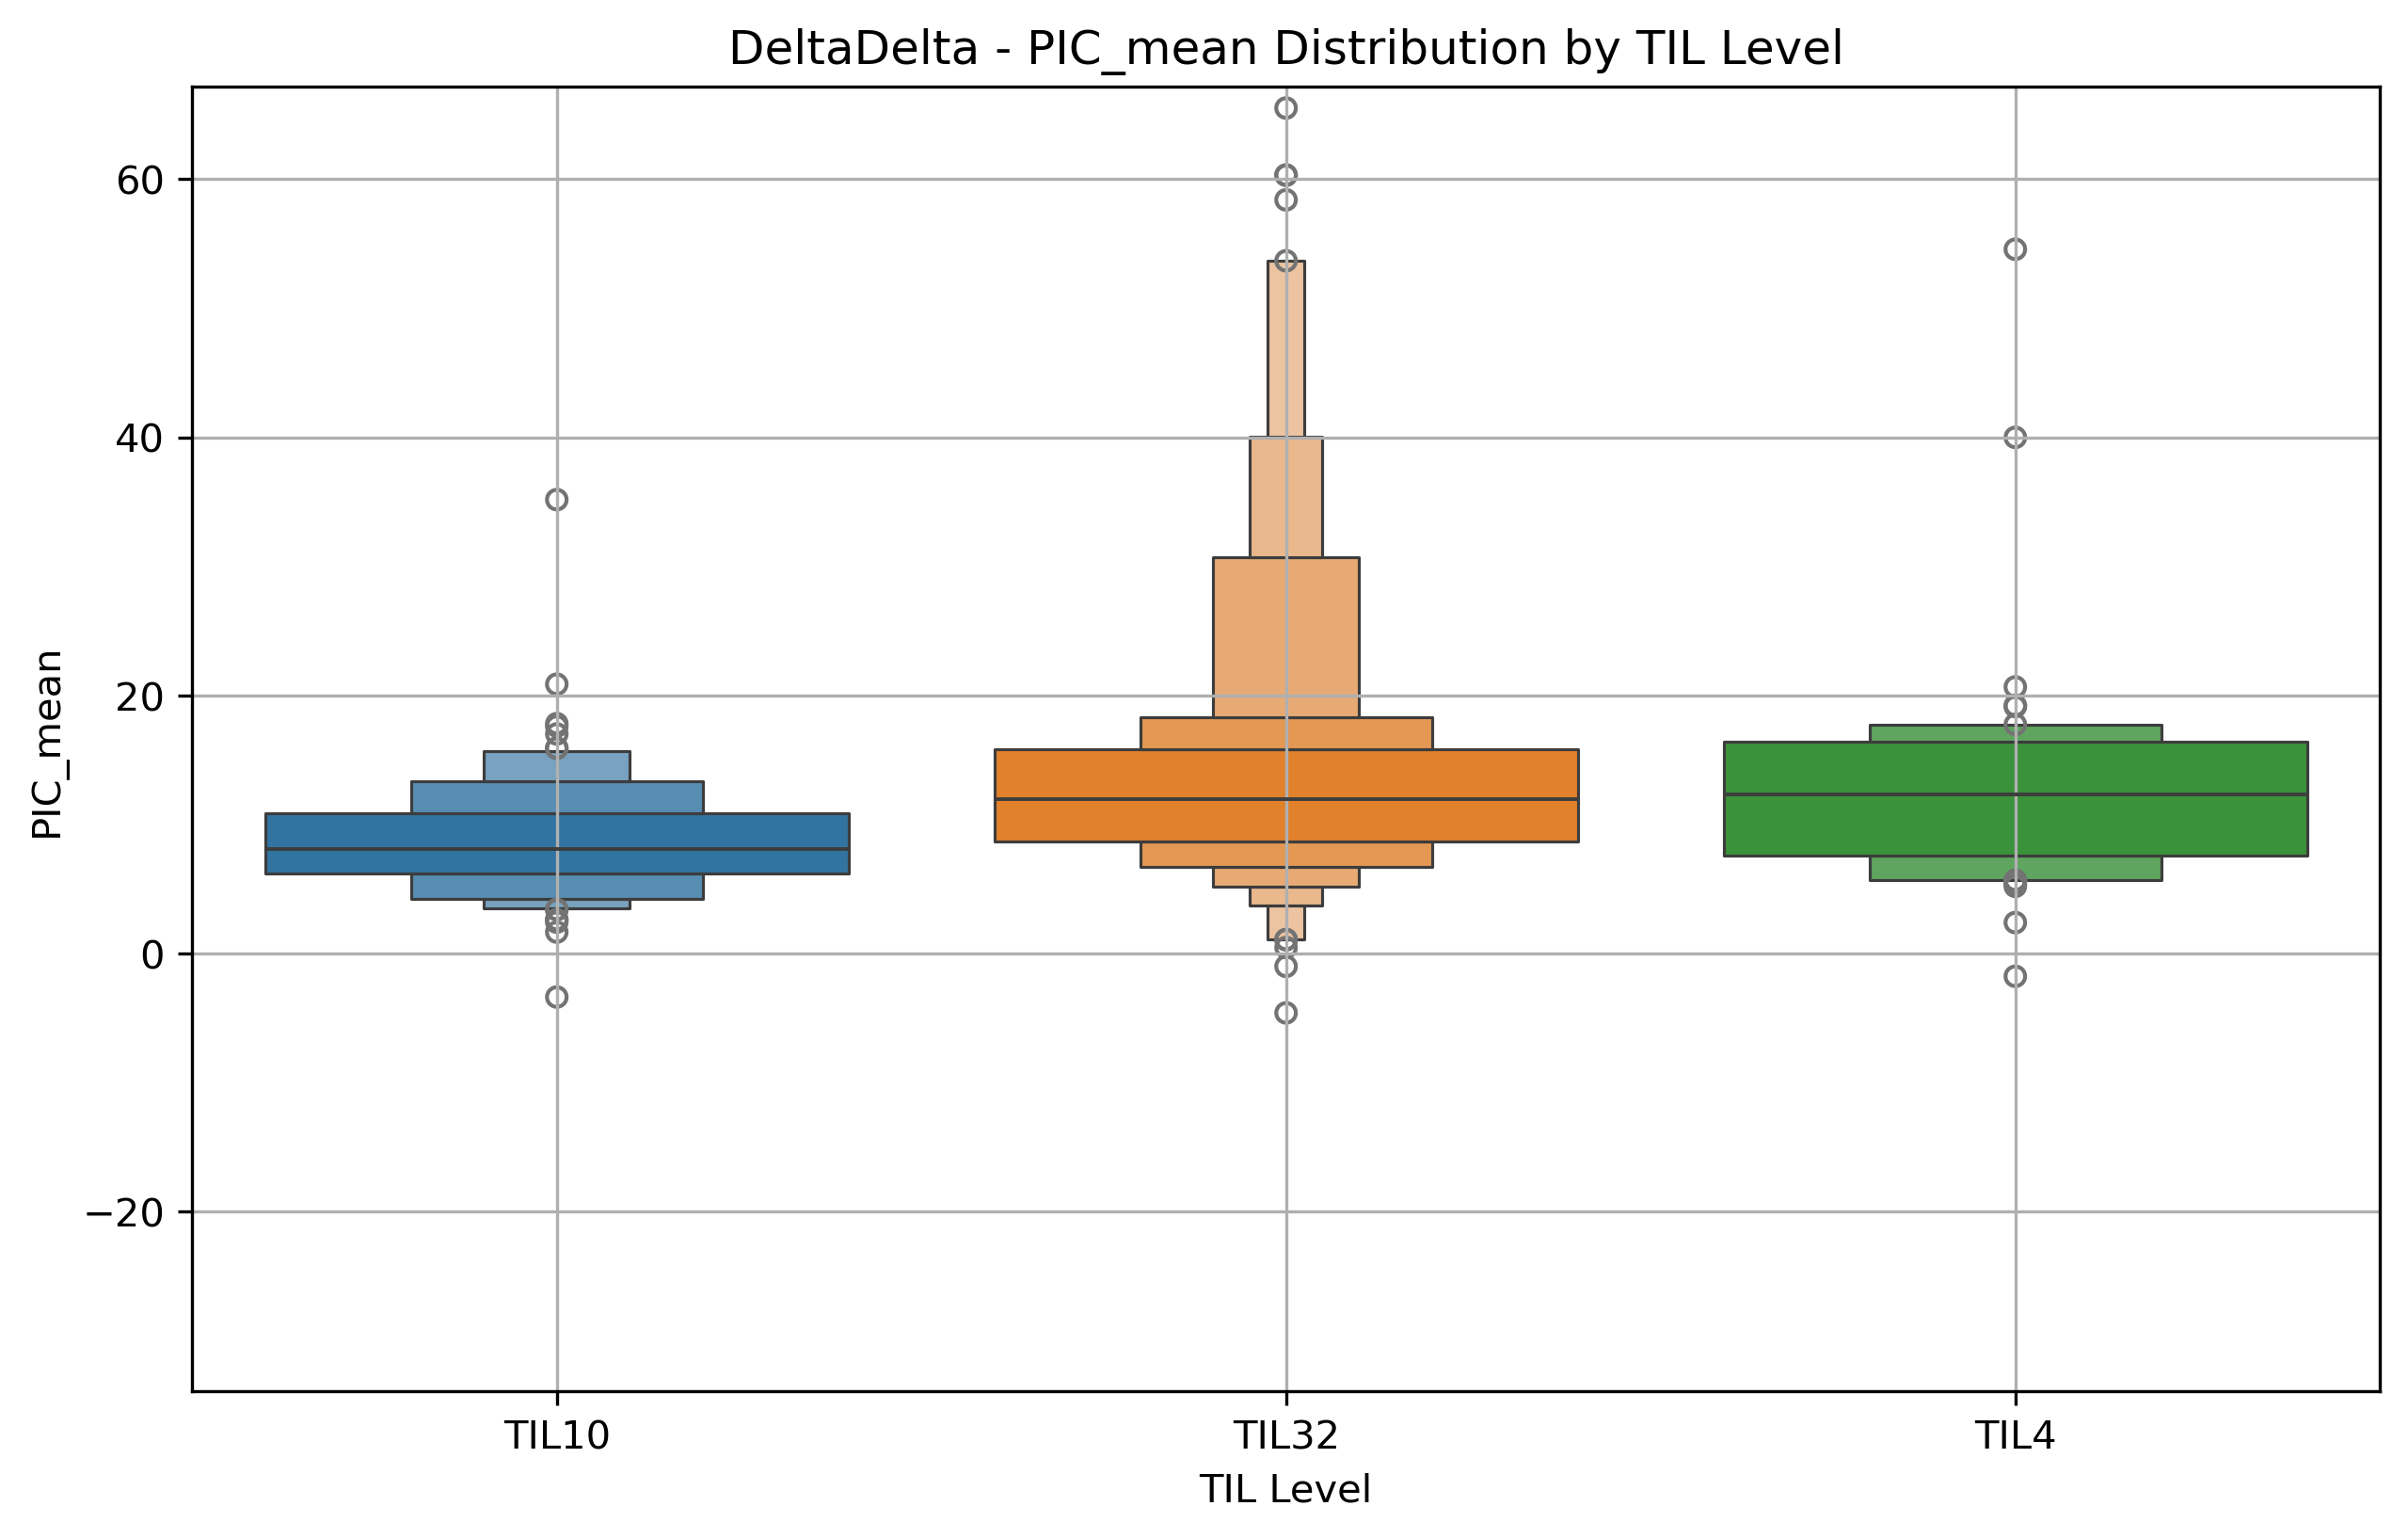
\includegraphics[width=0.8\textwidth]{pictures/fig12_ICPTIL.png}
    \caption{ICP trend in different TIL} % Add a meaningful caption
    \label{fig:ICPTIL} % Add a label for referencing
\end{figure}

\begin{figure}[h!]
    \centering
    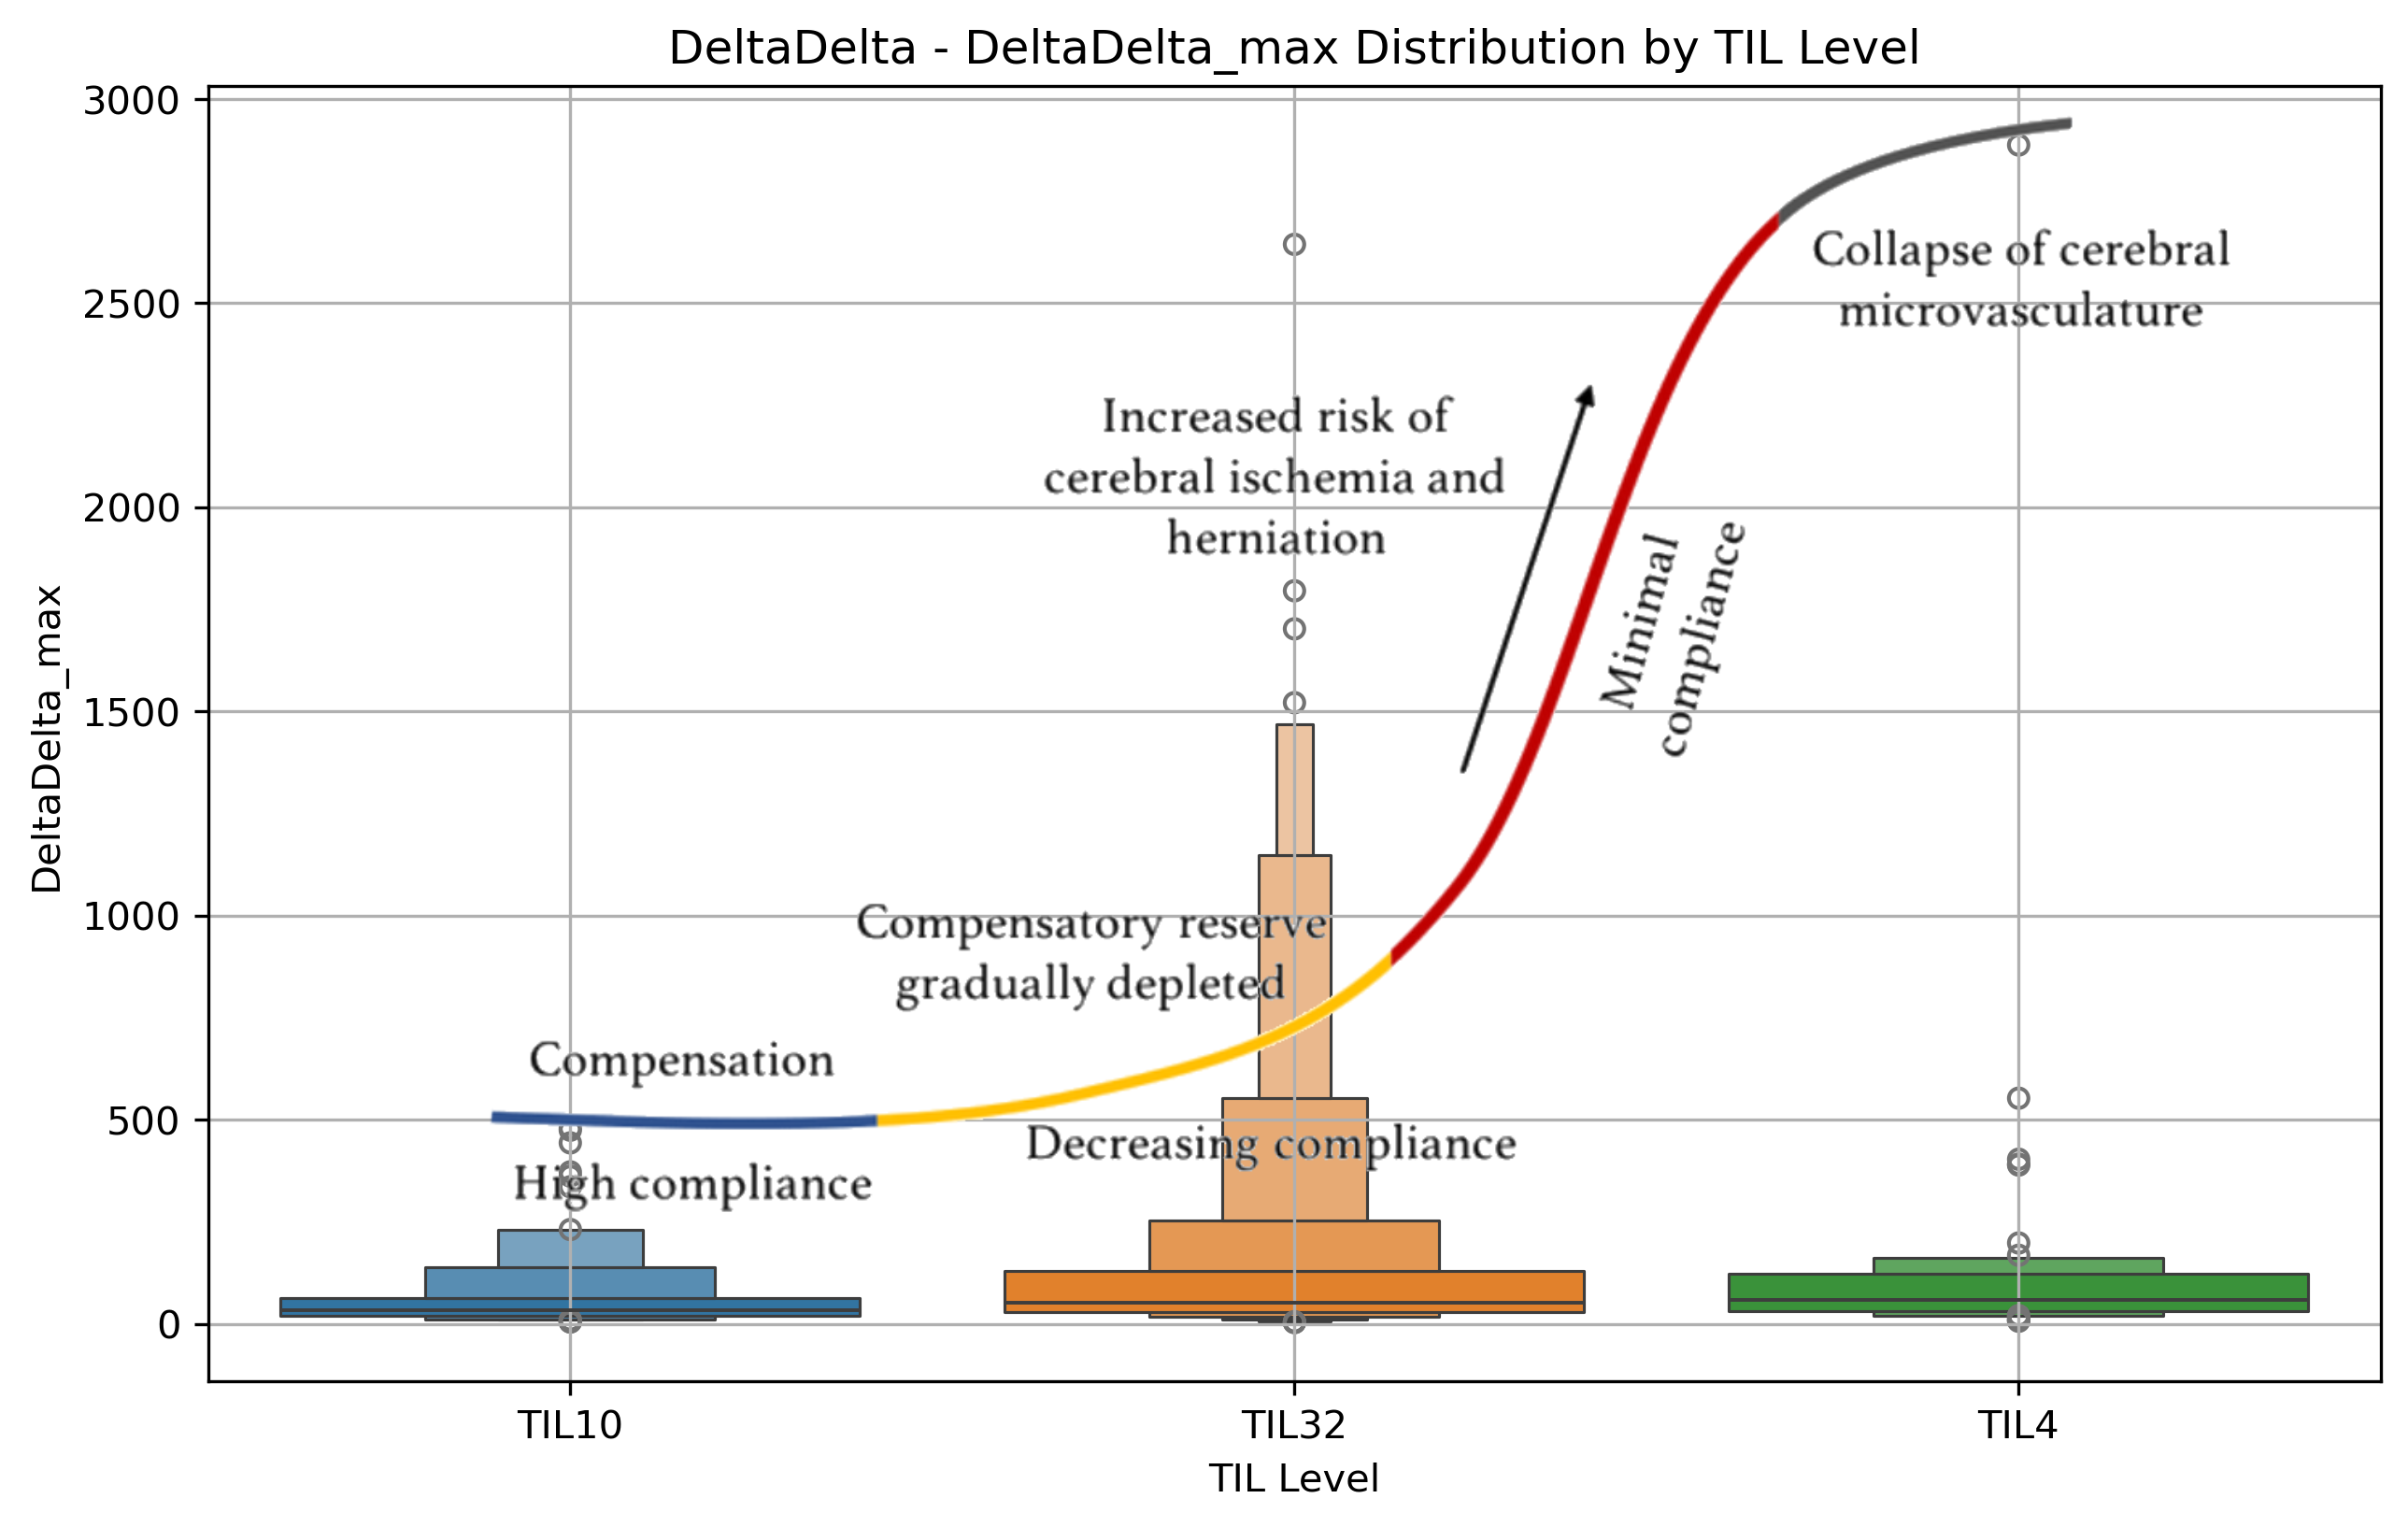
\includegraphics[width=0.8\textwidth]{pictures/fig13_DDTIL.png}
    \caption{DeltaICP/DeltaNa and cerebral compliance} % Add a meaningful caption
    \label{fig:DDTIL} % Add a label for referencing
\end{figure}


\section{Discussion}
%key findings temp title
We found that  serum sodium fluctuations and relative ICP fluctuations, are a significant predictor of mortality, in line with findings from Harrois et. al.\cite{harroisVariabilitySerumSodium2021a}

In our study, even after adjusting for baseline severity, fluctuations in serum sodium and ICP, even within normal ranges, were still linked to 14-day mortality.

The DeltaICP/DeltaNa ratio suggests that larger fluctuations in serum sodium are associated with the need for higher therapy intensity levels, raising the possibility that acute sodium variations may partially explain the relationship between DeltaICP/DeltaNa and patient outcomes.\\

%discussione vera e propria
Severe dysnatremia has long been associated with higher mortality rates. Sodium disorders are often caused by excessive administration or restriction of free water, but they are also linked to various comorbidities. Additionally, treatments such as surgery\cite{marshallAssociationSodiumFluctuations2017}\cite{sakrFluctuationsSerumSodium2013}, trauma or other acute illnesses\cite{senSodiumVariabilityAssociated2017a} can trigger or exacerbate these imbalances.

However, emerging evidence\cite{darmonPrognosticConsequencesBorderline2013} indicates that even mild deviations from normal sodium levels or simple fluctuations in sodium values may also carry significant clinical implications, especially in the brain injured patient. While this is well documented in subarachnoid hemorrhage \cite{jinAssociationSerumSodium2022}\cite{labibSodiumItsImpact2024}\cite{balesEffectHyponatremiaSodium2016}\cite{topjianGreaterFluctuationsSerum2014}\cite{eaglesSignificanceFluctuationsSerum2019}\cite{haradaImpactHormonalDynamics2022}, the effect on TBI has only recently been explored\cite{harroisVariabilitySerumSodium2021a}.

%non sono sicuro di questa frase
Our findings are significant for several reasons. First, understanding the risk factors associated with mortality helps clinicians make informed decisions about how often to monitor sodium levels, the type of fluids administered (hypotonic vs. isotonic), and how much sodium levels are allowed to fluctuate. Second, identifying sodium fluctuations as an independent risk factor for hospital mortality highlights the need to further explore their physiological causes and impacts, which could help clinicians identify at-risk patients earlier and potentially reduce mortality rates.

In our DeltaICP/DeltaNa analysis, we found that larger fluctuations in DeltaICP/DeltaNa were associated with higher mortality, this could be driven by DeltaNa alone. Rapid changes in sodium levels over a short time may pose a greater risk to patients due to the fast cerebral fluid shifts that occur. In response to hypertonic conditions in the extracellular space, brain cells attempt to restore osmotic balance by absorbing organic osmoles, a process that requires time. Sudden shifts in extracellular sodium can lead to intracellular fluid and electrolyte imbalances, resulting in cellular edema, particularly in an already injured brain with compromised or slower adaptive mechanisms. Additionally, it remains challenging to determine how our interventions might affect the unsalvageable brain—could our therapies inadvertently harm the very salvageable brain tissue we aim to protect in the first place?

%TIL
It’s plausible that patients who died or had poor neurological outcomes at 14 days were exposed to a broader range of sodium concentrations due to the need for therapies like hypertonic saline. Although the delta/delta ratio is a relative measurement, the overall variation appears low. This counterintuitive result could be attributed to minimal fluctuation occurring at consistently high levels of Na (as part of the therapeutic strategy) and ICP (due to exhausted cerebral compliance).
%inserire qui grafico sovrapposto di curva compliance e TIL.

%parlando di TIL, specificare come le distribuzioni dei nostri pazienti siano sovrapponibili con quelle di altri studi: es SYANPSE-ICU

\subsection{Limitations and current prospectives}
This is a retrospective study, and as such, it carries the inherent limitations associated with this type of research.

We did not assess neurological outcomes nor the Glasgow Outcome Coma Scale was available in our database. This limitation should be addressed in future studies investigating sodium fluctuations in TBI patients.

We didn't assessed the impact of intravenous fluid administration on sodium variability, as it was challenging to extract detailed information regarding the specific types of hypertonic saline\cite{holdenHypertonicSalineUse2023a} used for osmolar therapy.
For similar reasons, we didn't assessed the impact of diabete insipidus through desmopressin administration, as considering it alone as a surrogate marker woulnd't have been enough to diagnose DI or to discriminate with other brain-related plasma sodium disorders (SIADH or CSW). 

Although we adjusted for TIL, serum sodium fluctuations may still be a reflection of overall illness severity. Nevertheless, dysnatremias remain a known risk factor and should be incorporated into future predictive models for mortality in TBI patients, including fluctuations within normal limits, rather than dismissed as a mere consequence of disease severity.

Additional limitations in the subanalysis of patients within TIL therapy categories, beyond the already mentioned hypertonic saline, include missing data on decompressive craniectomy\cite{kimRecentUpdatesControversies2023a} and other interventions that are difficult to associate with specific treatment goals. For instance, it’s unclear whether vasopressors were used to manage elevated ICP or for other hemodynamic purposes, further complicating the analysis.

Lastly, patients who died within the first three days were excluded, which may limit the generalizability of our results.

\textcolor{red}{frasi da inserire: model 2 tiene conto di Dose Na e Dose ICP, in parte l'effetto è ridondante, essendo che parte della Dose Na causa Dose ICP ma è anche vero che la Dose NA data dalla ipernatriemia dovrebbe essere protettiva. Altro punto: la dose ICP dei pazienti con WOLST ha effetto tautologico (vedi arturo)}


\section{Conclusion}
While doses of potassium, glucose, and water are routinely adjusted, sodium is typically administered at standard concentrations as long as serum levels remain within an acceptable or desired range. This is common practice in many ICU patients and is well tolerated in most cases. However, for some individuals, the sodium content may not align with their intravascular volume or neuroendocrine status, leading to impaired sodium homeostasis. Until it is definitively proven that dysnatremia is merely a non-causal marker of an underlying harmful systemic process, it is prudent to assume that even slight sodium fluctuations and the resulting osmotic shifts could be detrimental. Therefore, the focus should perhaps shift to sodium fluctuations, or even osmolality. Minimizing sodium fluctuations to maintain a stable sodium trajectory and osmolality might be of more importance than sodium levels themselves.






\clearemptydoublepage


%%%% TAIL OF THE DOCUMENT
\backmatter
%list of figures
\listoffigures
\clearemptydoublepage
%list of tables
\listoftables
\clearemptydoublepage
%bibliography
\addcontentsline{toc}{chapter}{Bibliography}
\bibliography{bibliography/bibThesis}
\bibliographystyle{abbrv}
\clearemptydoublepage

\end{document}

